\RequirePackage[l2tabu,orthodox]{nag}
\documentclass[12pt,oneside,article,draft]{memoir}
% !TEX root = ./CCC_Note.tex

\usepackage{amsmath}
\usepackage{amsthm}
\usepackage{amsfonts}
\usepackage{amssymb}
\usepackage{mathtools}
%\usepackage{datetime}
\usepackage[usenames,dvipsnames]{xcolor}
\usepackage[bookmarks=true,colorlinks=true, linkcolor=MidnightBlue, citecolor=cyan]{hyperref}
\usepackage[T1]{fontenc}
\usepackage[sc]{mathpazo}
\linespread{1.05}
\usepackage{mathrsfs}
\usepackage{euscript}
%\usepackage{MnSymbol}
\usepackage{paralist}
\usepackage{todonotes}
\usepackage{makecell}
\usepackage{booktabs}
\usepackage{tikz}
\usetikzlibrary{cd}
\usepackage{tensor}

\usetikzlibrary{decorations.markings,arrows.meta,calc,fit,quotes}
\hypersetup{final}

\DeclareMathOperator{\id}{id}
\DeclareMathOperator{\dom}{dom}
\DeclareMathOperator{\cod}{cod}
\DeclareMathOperator{\dvert}{Vert}
\DeclareMathOperator{\Lax}{Lax}
\DeclareMathOperator{\Hom}{Hom}
\DeclareMathOperator{\Ob}{Ob}
\DeclareMathOperator{\Tr}{Tr}


\theoremstyle{plain}
\newtheorem{theorem}{Theorem}[section]
\newtheorem*{theorem*}{Theorem}
\newtheorem{proposition}[theorem]{Proposition}
\newtheorem{corollary}[theorem]{Corollary}
\newtheorem{lemma}[theorem]{Lemma}
\newtheorem*{lemma*}{Lemma}

\theoremstyle{definition}
\newtheorem{definition}[theorem]{Definition}
\newtheorem{exercise}{Exercise}[section]

\theoremstyle{remark}
\newtheorem{example}[theorem]{Example}
\newtheorem{remark}[theorem]{Remark}

\newcommand{\prodb}{\mathbin{\Pi}}
\newcommand{\iso}{\cong}

\newcommand{\cat}[1]{\mathscr{#1}}
\newcommand{\Cat}[1]{\mathbf{#1}}
\newcommand{\fun}[1]{#1}
\newcommand{\Fun}[1]{\mathsf{#1}}
%\newcommand{\hom}{\mathrm{hom}}
\newcommand{\twocat}[1]{\mathcal{#1}}
\newcommand{\dblcat}[1]{\mathbb{#1}}
\newcommand{\Mon}{\Cat{Mon}}
\newcommand{\Prof}{\Cat{Prof}}
\newcommand{\MProf}{\Cat{MProf}}
\newcommand{\MonCat}{\Cat{MonCat}}
\newcommand{\SymMonCat}{\Cat{SymMonCat}}
\newcommand{\CompCat}{\Cat{CompCat}}
\newcommand{\TrCat}{\Cat{TrCat}}
\newcommand{\Set}{\Cat{Set}}
\newcommand{\Int}{\Fun{Int}}

\newcommand{\op}[1]{{#1}^{\text{op}}}
\newcommand{\vop}[1]{{#1}^{\text{vop}}}
\newcommand{\hop}[1]{{#1}^{\text{hop}}}

\newcommand{\Alg}{\mathrm{Alg}}
\newcommand{\Coalg}{\mathrm{Coalg}}
\newcommand{\RAlg}[1][]{\mathbb{R}_{#1}\text{-}\Alg}
\newcommand{\LCoalg}[1][]{\mathbb{L}_{#1}\text{-}\Coalg}
\newcommand{\LCoalgA}{\mathbb{L}_1\text{-}\Coalg}
\newcommand{\LCoalgB}{\mathbb{L}_2\text{-}\Coalg}

\newcommand{\twocell}[3][]{\arrow[draw=none,to path={(dom#2.center)--(cod#2.center)\tikztonodes}]{}[anchor=center,#1]{\Downarrow #3}}
\newcommand{\twocellalt}[3][]{\arrow[draw=none,to path={(dom#2.center)--(cod#2.center)\tikztonodes}]{}[anchor=center,#1]{#3}}
\newcommand{\twocellA}[2][]{\twocell[#1]{A}{#2}}
\newcommand{\twocellB}[2][]{\twocell[#1]{B}{#2}}
\newcommand{\twocellC}[2][]{\twocell[#1]{C}{#2}}
\newcommand{\twocellD}[2][]{\twocell[#1]{D}{#2}}
\newcommand{\twocellE}[2][]{\twocell[#1]{E}{#2}}
\newcommand{\twocellF}[2][]{\twocell[#1]{F}{#2}}



\tikzcdset{
	arrow style=tikz,
	diagrams={>={Classical TikZ Rightarrow[angle=63:4pt, line width=.6pt]}},
	arrows={semithick}
}

\tikzset{tick/.style={postaction={decorate,decoration={markings,mark=at position 0.5 with {\draw[-] (0,.4ex) -- (0,-.4ex);}}}}}
\tikzset{dom/.style={append after command={coordinate[alias=dom#1]}},
		domA/.style={dom=A}, domB/.style={dom=B},
		domC/.style={dom=C}, domD/.style={dom=D},
		domE/.style={dom=E}, domF/.style={dom=F}}
\tikzset{cod/.style={append after command={coordinate[alias=cod#1]}},
		codA/.style={cod=A}, codB/.style={cod=B},
		codC/.style={cod=C}, codD/.style={cod=D},
		codE/.style={cod=E}, codF/.style={cod=F}}


\tikzset{
	%label/.style={font=\everymath\expandafter{\the\everymath\scriptstyle}},
	wiring diagram/.style={
		every to/.style={out=0,in=180,draw},
		label/.style={
			font=\everymath\expandafter{\the\everymath\scriptstyle},
			inner sep=0pt,
			node distance=2pt and -2pt},
		semithick,
		node distance=1 and 1,
		decoration={markings, mark=at position .5 with {\arrow{stealth};}},
		ar/.style={postaction={decorate}},
		execute at begin picture={\tikzset{
			x=\bbx, y=\bby,
			every fit/.style={inner xsep=\bbx, inner ysep=\bby}}}
		},
	bbx/.store in=\bbx,
	bbx = 1.5cm,
	bby/.store in=\bby,
	bby = 1.75ex,
	bb port sep/.store in=\bbportsep,
	bb port sep=2,
	% bb wire sep/.store in=\bbwiresep,
	% bb wire sep=1.75ex,
	bb port length/.store in=\bbportlen,
	bb port length=4pt,
	bb min width/.store in=\bbminwidth,
	bb min width=1cm,
	bb rounded corners/.store in=\bbcorners,
	bb rounded corners=2pt,
	bb small/.style={bb port sep=1, bb port length=2.5pt, bbx=.4cm, bb min width=.4cm, bby=.7ex},
	bb/.code 2 args={
		\pgfmathsetlengthmacro{\bbheight}{\bbportsep * (max(#1,#2)+1) * \bby}
		\pgfkeysalso{draw,minimum height=\bbheight,minimum width=\bbminwidth,outer sep=0pt,
			rounded corners=\bbcorners,thick,
			prefix after command={\pgfextra{\let\fixname\tikzlastnode}},
			append after command={\pgfextra{\draw
				\ifnum #1=0{} \else foreach \i in {1,...,#1} {
					($(\fixname.north west)!{\i/(#1+1)}!(\fixname.south west)$) +(-\bbportlen,0) coordinate (\fixname_in\i) -- +(\bbportlen,0) coordinate (\fixname_in\i')}\fi
				\ifnum #2=0{} \else foreach \i in {1,...,#2} {
					($(\fixname.north east)!{\i/(#2+1)}!(\fixname.south east)$) +(-\bbportlen,0) coordinate (\fixname_out\i') -- +(\bbportlen,0) coordinate (\fixname_out\i)}\fi;
			}}}
	},
	bb name/.style={append after command={\pgfextra{\node[anchor=north] at (\fixname.north) {#1};}}}
}

\usetikzlibrary{arrows,calc,chains,matrix,positioning,scopes,snakes}


\newcommand{\vinp}[1]{\overline{\inp{#1}}}
\newcommand{\voutp}[1]{\overline{\outp{#1}}}
%\newcommand{\inp}[1]{#1^{\textnormal{in}}}
%\newcommand{\outp}[1]{#1^{\textnormal{out}}}
\newcommand{\inp}[1]{#1^-}
\newcommand{\outp}[1]{#1^+}

% \def\bhline{\Xhline{2\arrayrulewidth}}
% \def\bbhline{\Xhline{2.5\arrayrulewidth}}
\def\alg{{\text \textendash}\Cat{Alg}}
\def\XCat{\textnormal{$\Cat{X}$-$\Cat{Cat}$}}
\def\To{\xrightarrow}
\def\ul{\underline}
\def\List{\textnormal{List}}
\def\SList{\textnormal{SList}}
\def\SSList{\textnormal{SSList}}

\newcommand{\erase}[1]{{}}
\def\NN{\mathbb{N}}
\def\ss{\subseteq}
\def\boo{{\Ob\iso}}
\newcommand{\bo}{\mathsf{bo}}
\newcommand{\ff}{\mathsf{ff}}


\settrims{0pt}{0pt} % page and stock same size
\setlxvchars %calculate line length such that there are about 65 characters per line in \normalfont
\settypeblocksize{*}{36pc}{*} % {height}{width}{ratio}
\setlrmargins{*}{*}{1} % {spine}{edge}{ratio}
%\setulmargins{*}{*}{1} % {upper}{lower}{ratio}, hight of typeblock fixed
\setulmarginsandblock{1in}{1in}{*} % hight of typeblock computed
\setheadfoot{\onelineskip}{2\onelineskip} % {headheight}{footskip}
\setheaderspaces{*}{1.5\onelineskip}{*} % {headdrop}{headsep}{ratio}
\checkandfixthelayout

\setcounter{tocdepth}{2}
\setcounter{secnumdepth}{2}
\pagestyle{companion}
\renewcommand*{\chaptitlefont}{\bfseries\Large}
\setsecheadstyle{\bfseries\large\raggedright}
\setsubsecheadstyle{\bfseries\raggedright}

\title{String diagrams for traced categories are oriented 1-cobordisms}
\author{
   David I. Spivak
      \thanks{Spivak and Schultz were supported by AFOSR grant FA9550--14--1--0031, ONR grant N000141310260, and NASA grant NNH13ZEA001N.}
   \and Patrick Schultz${}^*$%\footnotemark[1]
   \and Dylan Rupel
}


\begin{document}
\tightlists
\firmlists

\maketitle
\begin{abstract}
   We give an alternate conception of string diagrams as 1-dimensional oriented cobordisms, the
   operad of which we denote by $\Cob$. The axioms of traced categories are fully encoded by $\Cob$
   in the sense that there is an equivalence between $\Cob$-algebras and
   traced categories. We also prove a substantial generalization of this fact which characterizes
   lax functors out of compact or traced categories. 
\end{abstract}
Global todo's:
\begin{enumerate}
   \item Uncomment the $\backslash${listoftodos} command in latex below.
   \item Add keywords: Traced categories, compact categories, lax functors, equipments, monoidal categories, operads, factorization systems.
\end{enumerate}
%\listoftodos

\setcounter{tocdepth}{1}
\tableofcontents*

\chapter{Introduction}

Traced symmetric monoidal categories, hereafter \emph{traced categories}, have been used to model
processes with feedback~\cite{Abramsky1} or operators with fixed points~\cite{PontoShulman}. A
graphical calculus for traced categories was developed by Joyal, Street, and
Verity~\cite{JoyalStreetVerity}, in which string diagrams of the form
\begin{equation}\label{dia:string_diagram}
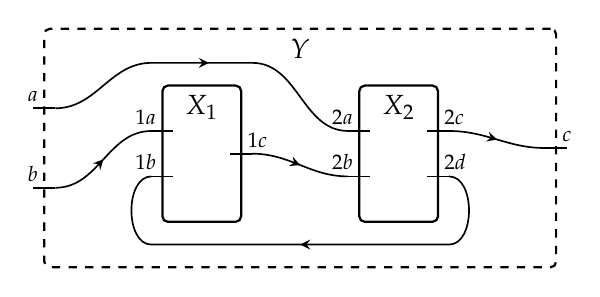
\begin{tikzpicture}[wiring diagram]
   \node[bb={2}{1}, bb name=$X_1$] (X1) {};
   \node[bb={2}{2}, right=of X1, bb name=$X_2$] (X2) {};
   \node[bb={2}{1}, dashed, fit={(X1) (X2) ($(X1.north)+(0,1.5)$) ($(X1.south)-(0,1)$)},
            bb name=$Y$] (Y) {};
   \draw[label]
      node[above left=of Y_in1]     {$a$}
      node[above left=of Y_in2]     {$b$}
      node[above right=of Y_out1]   {$c$}
      node[above left=of X1_in1]    {$1a$}
      node[above left=of X1_in2]    {$1b$}
      node[above right=of X1_out1]  {$1c$}
      node[above left=of X2_in1]    {$2a$}
      node[above left=of X2_in2]    {$2b$}
      node[above right=of X2_out1]  {$2c$}
      node[above right=of X2_out2]  {$2d$};
   \draw[ar] (Y_in2') to (X1_in1);
   \draw[ar] (X1_out1) to (X2_in2);
   \draw[ar] (X2_out1) to (Y_out1');
   \draw[ar] let \p1=(X1.north west), \p2=(X1.north east), \n1={\y1+\bby}, \n2=\bbportlen in
      (Y_in1') to (\x1-\n2,\n1) -- (\x2+\n2,\n1) to (X2_in1);
   \draw[ar] let \p1=(X2.south east), \p2=(X1.south west), \n1={\y1-\bby}, \n2=\bbportlen in
      (X2_out2) to[in=0] (\x1+\n2,\n1) -- (\x2-\n2,\n1) to[out=180] (X1_in2);
\end{tikzpicture}
\end{equation}
represent compositions. That is, new morphisms are constructed from old by specifying which outputs
will be fed back into which inputs. In fact, these are related to Penrose diagrams in $\ncat{Vect}$, and the word \emph{traced} originates in
this vector space terminology~\cite{JoyalStreetVerity}.

\section{Traced string diagrams as cobordisms}\label{sec:traced_string_cob}

A string diagram usually does not explicitly include the outer box $Y$. If we include it, as in
(\ref{dia:string_diagram}), the resulting \emph{wiring diagram} can be given another interpretation:
it represents a 1-dimensional cobordism between oriented 0-manifolds. For example, the box $X_1$ in
the picture includes only the data of a pair of finite sets,
$(\inp{X_1},\outp{X_1})=(\{1a,1b\},\{1c\})$, which can be interpreted as an oriented 0-manifold.
Moreover, the wiring diagram itself, in which boxes $X_1,\ldots,X_n$ are wired together inside a
larger box $Y$, can be interpreted as an oriented cobordism from $X_1\sqcup\cdots\sqcup X_n$ to $Y$.
This is a morphism in the (colored) operad $\Cob$, underlying the symmetric monoidal category of
oriented 1-cobordisms; see Section~\ref{sec:wds_and_cob}.

There is actually a bit more data in a string (or wiring) diagram for a traced category $\cat{C}$ than in a cobordism.
Namely, each input and output of a box must be labeled by an object of $\cat{C}$ and the wires connecting boxes must respect the labels (e.g., in (\ref{dia:string_diagram}) object 2d must equal object 1b). We will thus consider the operad $\LCob{\LabSet}$ of oriented 1-dimensional cobordisms over a fixed set $\LabSet$ of labels.

In the table below, we record these two interpretations of a string diagram. Note the ``degree
shift'' between the second and third columns.
\begin{center}
\begin{tabular}{lll}
   \toprule
      \multicolumn{3}{c}{Interpretations of string diagrams} \\
   \midrule
      String diagram & Traced category $\cat{C}$ & $\LCob{\LabSet}$ \\
   \midrule
      Wire label set, $\LabSet$ & Objects, $\LabSet\coloneqq\Ob(\cat{C})$ & Label set, $\LabSet$ \\
      Boxes, e.g., \tikz[wiring diagram,bb port sep=1,bby=2.4pt,bb min width=5.5pt,
                  bb port length=2pt,bb rounded corners=1pt,baseline=(B.south)]
               {\node[bb={1}{2}] (B) {};}
         & Morphisms in $\cat{C}$& Objects (oriented 0-mfds over $\LabSet$) \\
      String diagrams & Compositions in $\cat{C}$& Morphisms (cobordisms over $\LabSet$) \\
      Nesting & Axioms of traced cats & Composition (of cobordisms) \\
   \bottomrule
\end{tabular}
\end{center}

\subsection{The formal connection between Cob-algebras and Traced categories}
   \label{sec:statement_of_main_thm}

The relationship between these interpretations of string diagrams is most easily made precise when
the set $\LabSet$ of labels is fixed. Let $\TTrCat$ denote the 2-category of traced categories,
strong traced functors, and monoidal natural isomorphisms \cite{HK}, and let $\TrCat$ denote its
underlying 1-category.%
\footnote{
   We use a similar notational convention throughout this paper. We denote named 1-categories,
   monoidal categories, and operads with bold roman letters, e.g., $\ncat{Cob}$, and unnamed
   1-categories with script, e.g., $\cat{C}$. For named 2-categories or bicategories we do almost
   the same, but change the font of the first letter to calligraphic, such as $\nncat{T}{rCat}$; for
   unnamed 2-categories we use (unbold) calligraphic, e.g., $\ccat{D}$. Finally, for equipments
   (special double categories, see Section~\ref{sec:background_equipments}) we make the first letter
   blackboard bold, whether named (e.g., $\ndcat{P}{rof}$) or unnamed (e.g., $\dcat{D}$). The
   objects in a category, 2-category, or double category will be denoted with the usual math font
   (e.g., $T\in\Ob\TrCat$).
}
Finally, let $\TrCat_{\LabSet}$ denote the subcategory in which the object set is fixed to be free
on the set $\LabSet$---which we call its label set---together with label-preserving maps. For any
monoidal category $\cat{M}$, we denote by $\cat{M}\alg=\ncat{Lax}(M,\Set)$ the category of lax
functors $\cat{M}\to\Set$. Then there is an equivalence of categories
\begin{equation}\label{eq:single_fiber}
   \LCob{\LabSet}\alg\equiv\TrCat_{\LabSet}.
\end{equation}
Some intuition for this statement will be given in Section~\ref{subsec:cobalg_and_trCat}, and it
will be generalized in \ref{thm:TheoremA} and proven as such in Section~\ref{sec:deducing}.

% \section{Lax functors out of compact categories}\label{subsec:main_results}

% While the motivation for this paper was to understand the relationship between 1-cobordisms and traced categories, our work has led us to conclude that a more central issue is to understand lax functors out of compact categories. These fit into a larger picture, known as \emph{equipments} or \emph{framed bicategories}, which we review in Section~\ref{sec:background_equipments}. 

% The category $\Lax(\cat{C},\Set)$ of lax set-valued functors out of a compact category $\cat{C}$ has interesting behaviors. For example, when $\cat{C}$ is free on a set $\LabSet$ of objects, lax functors can be identified with object-free traced categories, as in \eqref{eq:single_fiber}, or with object-free compact categories:
% \begin{equation*}
%  \LCob{\LabSet}\alg\equiv\CompCat_{\LabSet}.
% \end{equation*}
% \todo[inline]{Finish writing this section.}

\subsection{The main results}\label{subsec:main_results}

The equivalence (\ref{eq:single_fiber}) has two drawbacks: the object set of the traced category is
fixed, and it is assumed to be free. Much of the work in this paper is to relax these two
conditions. For the latter, we prove that the 2-category of traced categories is equivalent to that
of \emph{object-free} traced categories (see Corollary~\ref{cor:TrCat_ObjectFree}). For the former,
we first explain what kind of variance is appropriate.

Let $\cat{C}$ and $\cat{C}'$ be object-free traced categories, such that $\Ob(\cat{C})$ is the free
monoid on a set $\LabSet$ and $\cat{C}'$ is the free monoid on a set $\LabSet'$. A strong functor
$F\colon \cat{C}\to \cat{C'}$ sends each object in $\LabSet$ to the tensor product of finitely many
objects in $\LabSet'$; that is, it induces a function $\Ob F\colon\LabSet\to\TT(\LabSet')$, where
$\TT\colon\Set\to\Set$ is the free monoid monad. Let $\Set_{\TT}$ denote the Kleisli category of
this monad, so $\Ob F$ is identified with a morphism in $\Set_{\TT}$. The compact category $\Cob/\LabSet$ is functorial in $\LabSet\in\Set$, and we will show later that this functor extends to functors
$$(\LCob{\bullet})\colon\Set_{\TT}\to\CompCat\qquad\tn{and}\qquad(\LCob{\bullet})\colon\Set_{\TC}\to\CompCat$$ 
(see~\eqref{dia:TMvsFrMonCat} and~\eqref{eqn:FMC}),
\todo{Patrick: check this paragraph; is $(\LCob{\bullet})$ clear enough notation?}%
and we can compose it with $\Lax(-,\Set)$ to obtain a functor which we denote
\begin{equation}\label{eqn:cob/bullet}
  (\LCob{\bullet})\alg\colon\Set_{\TT}^{\mathrm{op}}\too\Cat.
\end{equation}
By applying the Grothendieck construction to (\ref{eqn:cob/bullet}), we collect the equivalences
(\ref{eq:single_fiber}) for varying $\LabSet$ into a single functor, which is close to being an equivalence (see \ref{thm:TheoremA}). The same result holds when $\TT$ is replaced by $\TC$, the free compact category monad. The proof of the following result can be found in Section~\ref{sec:deducing}.

\begin{named}{Theorem A}\label{thm:TheoremA}
  There is a fully faithful functor of 1-categories
  \begin{equation*}
     \int^{\LabSet\in\Set_{\TT}}(\LCob{\LabSet})\alg \to \TrCat
  \end{equation*}
  such that the induced 2-functor $\int^{\LabSet\in\Set_{\TT}}(\LCob{\LabSet})\alg\to\TTrCat$ is 2-essentially surjective. 

  The above statements also hold when $\TT$ is replaced by $\TC$ and when $\TrCat$ and $\TTrCat$ are replaced by $\CompCat$ and $\CCompCat$.
\end{named}

\todo[inline]{And maybe a comment about the weird form of Theorem A, to the effect that we shouldn't
expect algebras of operads to be able to encode 2-cells.}

% \section{Generalization: Lax algebras on compact categories}

The definition of compact closed symmetric monoidal category, hereafter \emph{compact category}, can
be found in Section~\ref{sec:compact_and_int}, or in~\cite{MacLane}. Let $\CompCat$ denote the
category of compact categories and strong monoidal functors between them. We will see
(\ref{thm:orthogonal} and \ref{prop:CompProf_exact}) that there is a factorization system on
$\CompCat$, in which the left class consists of bijective-on-objects functors and the right class
consists of fully faithful functors. Let $\CompCat^{\bo}$ be the full subcategory of the arrow
category $\CompCat^{\to}$ spanned by the bijective-on-objects functors.

We will also prove a generalization of Theorem~\ref{thm:TheoremA}, where instead of considering lax
functors out of categories of the form $\LCob{\LabSet}$---i.e.\ free compact categories---we
consider lax functors out of arbitrary compact categories. For a fixed compact category $\cat{C}$,
we have the equivalence of categories
\begin{equation}\label{eqn:lax_compcat_bo}
   \Lax(\cat{C},\Set)\iso\cat{C}/\CompCat^{\bo}.
\end{equation}
where $\cat{C}/\CompCat^{\bo}$ is the category of strong, bijective-on-objects functors from
$\cat{C}$ to another compact category, with the evident commutative triangles as morphisms.

One advantage of this generalization is that it is more straightforward to handle changing the
category $\cat{C}$. Namely, we will prove the following theorem:

\begin{named}{Theorem B}\label{thm:TheoremB}
   There is an equivalence of fibrations
   \begin{equation*}
      \begin{tikzcd}[column sep=-1.8em]
         \int\limits^{\mathclap{\cat{C}\in\CompCat}} \Lax(\cat{C},\Set)
               \ar[rr,"\equiv"] \ar[dr,two heads]
            && \CompCat^{\bo} \ar[dl,two heads,"\dom"] \\
         & \CompCat &
      \end{tikzcd}
   \end{equation*}
\end{named}
\todo[inline]{Combine Theorem B and Corollary B.}
Recall from~\cite{JoyalStreetVerity} that traced categories are full subcategories of compact
categories.  The Int construction, applied to a traced category $\cat{C}$, returns the smallest
compact category $\Int(\cat{C})$ of which it is a monoidal subcategory; we call $\Int(\cat{C})$ the
\emph{compact closure} of $\cat{C}$. We will recall these notions in Sections~\ref{sec:intuition_for_traced}~and~\ref{sec:compact_and_int}.

It turns out that if our compact category $\cat{C}$ is the compact closure of some traced category
$\cat{D}$, then~\ref{thm:TheoremB} lifts to a result about $\cat{D}$. We record this result
as~\ref{cor:CorollaryB}, from which~\ref{thm:TheoremA} follows. These are proved in
Section~\ref{sec:deducing}.

\begin{named}{Corollary B}\label{cor:CorollaryB}
   There is an equivalence of fibrations
   \begin{equation*}
      \begin{tikzcd}[column sep=-1em]
         \int\limits^{\mathclap{\cat{C}\in\TrCat}} \Lax(\Int(\cat{C}),\Set)
               \ar[rr,"\equiv"] \ar[dr,two heads]
            && \TrCat^{\bo} \ar[dl,two heads,"\dom"] \\
         & \TrCat &
      \end{tikzcd}
   \end{equation*}
\end{named}

We can give a better high-level story once we have reviewed equipments; see the introduction to Section~\ref{sec:equipments_monoidal_profunctors}. For the remainder of the introduction, we will attempt to build intuition.

\section{Wiring Diagrams, cobordisms, and traced categories}

In this section, we give a bit more intuition about the connection between wiring diagrams and cobordisms, and the equivalence between the category of traced categories
and the category of cobordism algebras.

\subsection{Wiring diagrams and $\Cob$}\label{sec:wds_and_cob}

The objects in $\Cob$ are signed sets $(\inp{X},\outp{X})$, each of which can be drawn as a box with
input wires $\inp{X}$ drawn entering the box, on its left, and output wires $\outp{X}$ drawn exiting
the box, on its right. We call the latter style \emph{an interface}.

\[
   \begin{tikzpicture}[node distance=0 and 0, baseline=(current bounding box.center)]
      \node (A1) {$-$};
      \node[below=-.1 of A1] (A2) {$-$};
      \node[below=-.1 of A2] (A3) {$-$};
      \node[below=-.1 of A3] (B1) {$+$};
      \node[below=-.1 of B1] (B2) {$+$};
   \end{tikzpicture}
   \hspace{4em}
   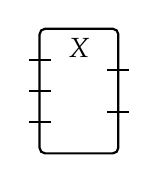
\begin{tikzpicture}[wiring diagram, bby=1.2ex, baseline=(current bounding box.center)]
      \node[bb={3}{2},bb name=$X$] {};
   \end{tikzpicture}
\]

Wiring diagrams seem to be a new way to visualize morphisms in the symmetric monoidal category
$\Cob$ of 1-dimensional oriented cobordisms. In fact, they are better suited to the operad associated to $\Cob$. The following shows the two approaches to drawing a 2-ary morphism $X_1,X_2\to Y$:

\[
   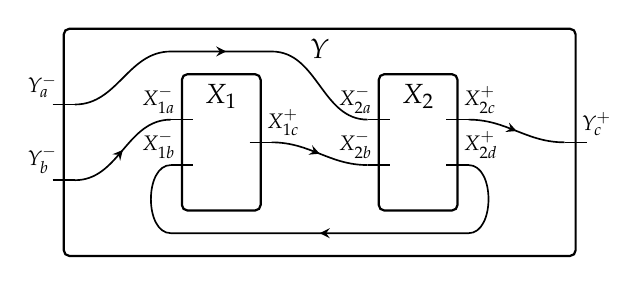
\begin{tikzpicture}[wiring diagram, baseline=(current bounding box.center)]
      \node[bb={2}{1}, bb name=$X_1$] (X1) {};
      \node[bb={2}{2}, right=of X1, bb name=$X_2$] (X2) {};
      \node[bb={2}{1}, fit={(X1) (X2) ($(X1.north)+(0,1)$) ($(X1.south)-(0,1)$)},bb name =$Y$] (Y) {};
      \draw[label]
          node[above left=of Y_in1]     {$\inp{Y}_a$}
          node[above left=of Y_in2]     {$\inp{Y}_b$}
          node[above right=of Y_out1]   {$\outp{Y}_c$}
          node[above left=of X1_in1]    {$\inp{X}_{1a}$}
          node[above left=of X1_in2]    {$\inp{X}_{1b}$}
          node[above right=of X1_out1]  {$\outp{X}_{1c}$}
          node[above left=2pt and -2pt of X2_in1]    {$\inp{X}_{2a}$}
          node[above left=of X2_in2]    {$\inp{X}_{2b}$}
          node[above right=of X2_out1]  {$\outp{X}_{2c}$}
          node[above right=of X2_out2]  {$\outp{X}_{2d}$};
      \draw[ar] (Y_in2') to (X1_in1);
      \draw[ar] (X1_out1) to (X2_in2);
      \draw[ar] (X2_out1) to (Y_out1');
      \draw[ar] let \p1=(X1.north west), \p2=(X1.north east), \n1={\y1+\bby}, \n2=\bbportlen in
          (Y_in1') to (\x1-\n2,\n1) -- (\x2+\n2,\n1) to (X2_in1);
      \draw[ar] let \p1=(X2.south east), \p2=(X1.south west), \n1={\y1-\bby}, \n2=\bbportlen in
         (X2_out2) to[in=0] (\x1+\n2,\n1) -- (\x2-\n2,\n1) to[out=180] (X1_in2);
   \end{tikzpicture}
   \qquad
   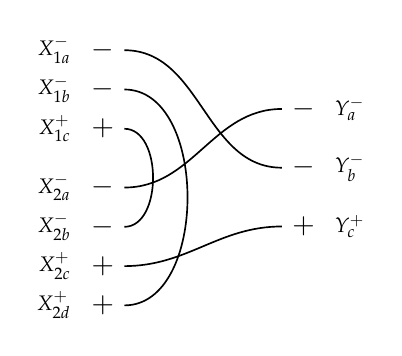
\begin{tikzpicture}[x=1cm,y=1ex,node distance=1 and 1,semithick,every label quotes/.style={font=\everymath\expandafter{\the\everymath\scriptstyle}},every to/.style={out=0,in=180},baseline=(current bounding box.center)]
      \node ["$\inp{X}_{1a}$" left] (X1a) {$-$};
      \node [below=0 of X1a, "$\inp{X}_{1b}$" left] (X1b) {$-$};
      \node [below=0 of X1b, "$\outp{X}_{1c}$" left] (X1c) {$+$};
      \node [below=1.5 of X1c, "$\inp{X}_{2a}$" left] (X2a) {$-$};
      \node [below=0 of X2a, "$\inp{X}_{2b}$" left] (X2b) {$-$};
      \node [below=0 of X2b, "$\outp{X}_{2c}$" left] (X2c) {$+$};
      \node [below=0 of X2c, "$\outp{X}_{2d}$" left] (X2d) {$+$};
      \node [below right=1.5 and 2 of X1a, "$\inp{Y}_a$" right] (Ya) {$-$};
      \node [below=1.5 of Ya, "$\inp{Y}_b$" right] (Yb) {$-$};
      \node [below=1.5 of Yb, "$\outp{Y}_c$" right] (Yc) {$+$};
      \draw (X1a) to (Yb);
      \draw (X1b) to[in=0] (X2d);
      \draw (X1c) to[in=0] (X2b);
      \draw (X2a) to (Ya);
      \draw (X2c) to (Yc);
   \end{tikzpicture}
\]

\subsection{$\Cob$-algebras and traced categories}\label{subsec:cobalg_and_trCat}

Here we sketch the equivalence of categories 
$$\LCob{\LabSet}\alg\equiv\TrCat_{\LabSet}$$
from Section~\ref{sec:statement_of_main_thm}. We will see that the same data are required, and the same conditions are
satisfied, whether one is specifying a lax functor $P\in\LCob{\LabSet}\alg$ or a traced category
$\cat{C}\in\TrCat_{\LabSet}$ with objects generated by $\LabSet$. 

First, for each box $X=(\inp{X},\outp{X})$ that might appear in a string diagram, both $P\colon\LCob{\LabSet}\to\Set$ and
$\cat{C}$ require a set, $P(X)$ and $\Hom_{\cat{C}}(\inp{X},\outp{X})$, respectively.
Second, for each string diagram, both $P$ and $\cat{C}$ require a function: an action on morphisms,
in the case of $P$, and a formula for performing the required compositions, tensors, and traces, in
the case of $\cat{C}$. The condition that $P$ is functorial corresponds to the fact that $\cat{C}$
satisfies the axioms of traced categories. 

We will briefly specifying how to construct a lax functor $P$ from a traced category $(\cat{C},\otimes,I,\Tr)$, whose objects are freely generated by $\LabSet$. We will abuse notation slightly as follows: Given a relative set
$\iota\colon Z\to\LabSet$, we will use the same symbol $Z$ to denote
the tensor $\bigotimes_{z\in Z}\iota(z)$ in $\cat{C}$. 

For an oriented 0-manifold $X=\inp{X}\sqcup \outp{X}$ over $\LabSet$, we
set $P(X)\coloneqq\Hom_{\cat{C}}(\inp{X},\outp{X})$. Given a cobordism $\Phi\colon X\to Y$, we need a function $P(\Phi)\colon P(X)\to P(Y)$. For any cobordism $\Phi$, there exist
$A,B,C,D,E\in\Ob\cat{C}$ such that $\inp{X}\cong C\otimes A$, $\outp{X}\cong C\otimes B$,
$\inp{Y}\cong A\otimes D$, $\outp{Y}\cong B\otimes D$, and $E$ is the set of floating loops in $\Phi$;
thus $\Phi$ is essentially equivalent to the cobordism shown on the right side of (\ref{eq:cob_and_trace_pic}).
\begin{equation}\label{eq:cob_and_trace_pic}
   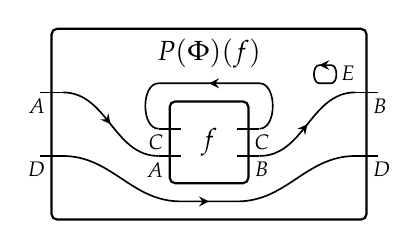
\begin{tikzpicture}[wiring diagram, bby=1.4ex, baseline=(current bounding box.center)]
      \node[bb port sep=1.5, bb={2}{2}] (domain) {$f$};
      \node[bb={2}{2}, fit={(domain) ($(domain.north)+(0,3)$) ($(domain.south)-(0,1)$)}, bb name=$P(\Phi)(f)$] (codomain) {};
      \draw[ar] (codomain_in1') to (domain_in2);
      \draw[ar] (domain_out2) to (codomain_out1');
      \draw[ar] let \p1=(domain.north east), \p2=(domain.north west), \n1={\y1+\bby}, \n2=\bbportlen in
          (domain_out1) to[in=0] (\x1+\n2,\n1) -- (\x2-\n2,\n1) to[out=180] (domain_in1);  %Trace on C
      \draw[ar] let \p1=(domain.south west), \p2=(domain.south east), \n1={\y1-\bby}, \n2=\bbportlen in
          (codomain_in2') to[in=180] (\x1+\n2,\n1) -- (\x2-\n2,\n1) to[out=0] (codomain_out2'); %Identity on D
      \draw[ar] let \p1=(domain.north east) in
          (\x1+.7*\bbx,\y1+\bby) to[in=0] (\x1+.7*\bbx,\y1+2*\bby) -- (\x1+.6*\bbx,\y1+2*\bby) to[out=180] (\x1+.6*\bbx,\y1+\bby) -- (\x1+.7*\bbx,\y1+\bby);%Loop
      \draw[label] let \p1=(domain.north east) in
          node[below left=of codomain_in1]     {$A$}
          node[below left=of codomain_in2]     {$D$}
          node[below right=of codomain_out1]    {$B$}
          node[below right=of codomain_out2]    {$D$}
          node[above left=.6 and 0 of codomain_out1']  {$E$}
          node[below left=of domain_in1]     {$C$}
          node[below left=of domain_in2]     {$A$}
          node[below right=of domain_out2]    {$B$}
          node[below right=of domain_out1]   {$C$};
   \end{tikzpicture}
   \qquad\qquad
   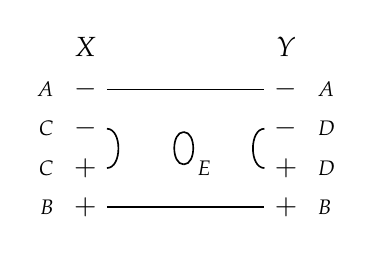
\begin{tikzpicture}[x=1cm,y=1ex,node distance=1 and 1,semithick,every label quotes/.style={font=\everymath\expandafter{\the\everymath\scriptstyle}},every to/.style={out=0,in=180},baseline=(current bounding box.center)]
      \node ["$A$" left] (X1a) {$-$};
      \node [above=0.25 of X1a] {$X$};
      \node [below=0 of X1a, "$C$" left] (X1b) {$-$};
      \node [below=0 of X1b, "$C$" left] (X2a) {$+$};
      \node [below=0 of X2a, "$B$" left] (X2b) {$+$};
      \node [right=2 of X1a, "$A$" right] (Y1a) {$-$};
      \node [above=0.25 of Y1a] {$Y$};
      \node [below=0 of Y1a, "$D$" right] (Y1b) {$-$};
      \node [below=0 of Y1b, "$D$" right] (Y2a) {$+$};
      \node [below=0 of Y2a, "$B$" right] (Y2b) {$+$};
      \node [right=1.45 of X2a, "$E$" left] {};
      \draw (X1a) to (Y1a);
      \draw (X1b) to[in=0] (X2a);
      \draw (X2b) to (Y2b);
      \draw (Y1b) to[in=180,out=180] (Y2a);
      \draw ($(X1b)+(1.25,-2.75)$) to[in=0] ($(X1b)+(1.25,-0.25)$);
      \draw ($(X1b)+(1.25,-0.25)$) to[in=180,out=180] ($(X1b)+(1.25,-2.75)$);
   \end{tikzpicture}
\end{equation}
With the above notation, for $f\in P(X)$ we can follow the string diagram (left of (\ref{eq:cob_and_trace_pic})) and define
\begin{equation}\label{eq:cob algebra formula}
   P(\Phi)(f)\coloneqq\Tr_{A,B}^C(f)\otimes D\otimes\Tr^E_{I,I}(\id_E).
\end{equation}


\section{Applications of the operadic perspective}

The operadic perspective on traced categories may be useful in concrete applications, such as for
modeling nested process diagrams. It may also be useful in pure mathematics, because the operad $\Cob$,
which indexes traced categories, can be easily modified to model a variety of other doctrines.
These two applications will be discussed in more detail in
Sections~\ref{sec:modular}~and~\ref{sec:math application} respectively.

\subsection{Modular design}\label{sec:modular}

When designing or investigating a complex system, it is often useful to think in terms of
interacting subsystems, put together to make a larger whole. In manufacturing, this is often called
\emph{modular design}. Each object in $\Cob$ represents an interface, or \emph{module}, with a
fixed number and type of inputs and outputs. The morphisms in $\Cob$ correspond to strategies by
which these interfaces can be wired together into a process, which itself has an interface.

An algebra $P\colon\Cob\to\Set$ provides semantics for these boxes (\cite{RupelSpivak},\cite{VagnerSpivakLerman}). For each interface $X$, the set
$P(X)$ represents the set of ``fillers'' for this interface. For example, one might imagine that
each interface $X$ can be filled by any state machine having that interface; in this case $P(X)$ is
the set of such state machines. For a morphism $\varphi\colon X_1,\ldots,X_n\to Y$, the function
$P(\varphi)$ tells us how to construct a filler of type $Y$, given fillers on each $X_i$.
Composition of cobordisms are drawn as nested diagrams:

\[
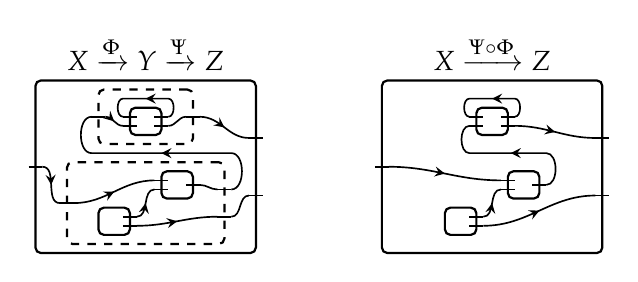
\begin{tikzpicture}[wiring diagram, bb small]
   \node[bb={2}{2}] (X1) {};
   \node[bb={1}{1}, fit={(X1) ($(X1.north)+(0,1)$)}, dashed] (Y1) {};
   \node[bb={2}{1}, below right=4 and 0 of X1] (X2) {};
   \node[bb={0}{2},below left=of X2] (X3) {};
   \node[bb={1}{2}, fit=(X2) (X3), dashed] (Y2) {};
   \node[bb={1}{2}, fit=(Y1) (Y2)] (Z) {};
   \draw[ar] (Z_in1') to (Y2_in1);
   \draw[ar] (Y2_in1') to (X2_in1);
   \draw[ar] (X3_out1) to (X2_in2);
   \draw[ar] (X3_out2) to (Y2_out2');
   \draw (Y2_out2) to (Z_out2');
   \draw[ar] (Y1_in1') to (X1_in2);
   \draw (X1_out2) to (Y1_out1');
   \draw[ar] (Y1_out1) to (Z_out1');
   \draw (X2_out1) to (Y2_out1');
   \draw[ar] let \p1=(Y2.north east), \p2=(Y1.south west), \n1={\y1+\bby}, \n2=\bbportlen in
      (Y2_out1) to[in=0] (\x1+\n2,\n1) -- (\x2-\n2,\n1) to[out=180] (Y1_in1);
   \draw[ar] let \p1=(X1.north east), \p2=(X1.north west), \n1={\y1+\bby}, \n2=\bbportlen in
      (X1_out1) to[in=0] (\x1+\n2,\n1) -- (\x2-\n2,\n1) to[out=180] (X1_in1);
   \node[anchor=south] at (Z.north) {$X\xrightarrow{\Phi}Y\xrightarrow{\Psi}Z$};

   \node[bb={2}{2}, right=10 of X1] (X1') {};
   \node[bb={2}{1}, below right=4 and 0 of X1'] (X2') {};
   \node[bb={0}{2},below left=of X2'] (X3') {};
   \node[bb={1}{2}, fit={($(X1'.north)+(0,1)$) (X2') (X3')}, inner xsep=2*\bbx, inner ysep=2*\bby] (Z') {};
   \draw[ar] (X3'_out1) to (X2'_in2);
   \draw[ar] (Z'_in1') to (X2'_in1);
   \draw[ar] (X1'_out2) to (Z'_out1');
   \draw[ar] (X3'_out2) to (Z'_out2');
   \draw[ar] let \p1=(X2'.north east), \p2=(X1'.south west), \n1={\y1+2*\bby}, \n2=\bbportlen in
      (X2'_out1) to[in=0] (\x1+\n2,\n1) -- (\x2-\n2,\n1) to[out=180] (X1'_in2);
   \draw[ar] let \p1=(X1'.north east), \p2=(X1'.north west), \n1={\y1+\bby}, \n2=\bbportlen in
      (X1'_out1) to[in=0] (\x1+\n2,\n1) -- (\x2-\n2,\n1) to[out=180] (X1'_in1);
   \node[anchor=south] at (Z'.north) {$X\xrightarrow{\Psi\circ\Phi}Z$};
\end{tikzpicture}
\]

In our model for modular design, any way to chunk the small boxes inside the big one will yield the
same result. This is a reflection of the functoriality of $P\colon\Cob\to\Set$, which says that
commutative diagrams in $\Cob$ are sent to commutative diagrams of sets. Nested structures, given
by composition of such morphisms, may be useful for the kind of chunking that humans use to
understand complex systems~\cite{Miller}.

\subsection{Mathematical application: varying the operad}\label{sec:math application}

Formalizing modular design using operads, as in~\cite{Spivak},~\cite{RupelSpivak}, and~\cite{VagnerSpivakLerman} was the original
motivation for the present paper, as the drawings had strong similarities to those found in traced
categories. However, it should be noted that none of these papers actually uses $\Cob$ as the
indexing category for their algebras. In fact, they use three different operads, of varying degrees
of similarity to $\Cob$. For example, there is an orthogonal factorization system on $\Cob$, for
which morphisms in the left class $\cat{L}$ include no closed loops, and the operad of interest in~\cite{VagnerSpivakLerman} is $\cat{L}$.

If one wished to make minor modifications in the axioms of traced categories to create some new sort of category $\ncat{Tr'Cat}$, one may proceed by imagining the string diagrams make sense in $\ncat{Tr'Cat}$. For example, one may want to consider cartesian traced categories, in which wires can split or terminate abruptly. Or they may want to allow splitting but not allow abrupt termination. 
\begin{center}
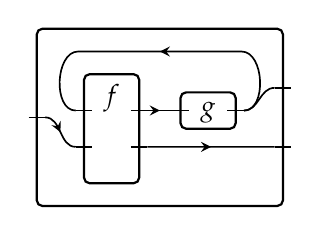
\begin{tikzpicture}[wiring diagram,bb min width =.7cm, bb port sep =1, bbx=.6cm,bb port length=3pt]
   \node[bb port sep=1.6, bb={2}{2}, bb name=$f$] (X1) {};
   \node[bb port sep=.8,bb={1}{1}, right=.7 of X1_out1, bb name=$g$] (X2) {};
   \node[bb={1}{2}, fit={(X1) (X2) ($(X1.north)+(0,1)$)}] (Y) {};
   \draw[ar] (Y_in1') to (X1_in2);
   \draw[ar,pos=.8] (X1_out1) to (X2_in1);
   \draw (X2_out1) to (Y_out1');
   \draw[ar] (X1_out2) to (Y_out2');
   \draw[ar] let \p1=(X2.north east), \p2=(X1.north west), \n1={\y2+\bby}, \n2=\bbportlen in
      (X2_out1) to[in=0] (\x1+.7*\n2,\n1) -- (\x2-.7*\n2,\n1) to[out=180] (X1_in1);
\end{tikzpicture}
\end{center}
We can accommodate the desired notion of string diagrams for $\ncat{Tr'Cat}$ by modifying the indexing operad $\Cob$ to some $\Cob'$. Using $\cat{L}$ for dynamical systems in \cite{VagnerSpivakLerman} is an example of this. As another, suppose that, as above, we want string diagrams in which wires can split but not terminate. Noting that an oriented cobordism $\varphi$ includes the data of a function
$$\varphi_1\colon\inp{X}\sqcup\outp{Y}\to\outp{X}\sqcup\inp{Y},$$ 
which is both injective and surjective, we can obtain the desired indexing operad $\Cob'$ by requiring surjectivity but not injectivity in $\varphi$.


\section{Plan of the paper} 

\todo[inline]{Write Plan.}

\section*{Acknowledgments}

Thanks go to Steve Awodey and Ed Morehouse for suggesting we formally connect the operad-algebra
picture in \cite{RupelSpivak} to string diagrams in traced categories. We also thank Mike Shulman for many useful conversations.

\chapter{Categorical preliminaries}\label{sec:traced categories}

In this section we remind the reader of some categorical preliminaries. Basic definitions and facts
about monoidal, traced, and compact categories, lax and strong functors, and the Int construction
are given in Sections~\ref{sec:prelim_monoidal}~through~\ref{sec:compact_and_int}. The fact that
the free compact category on a set has an algebraic description in terms of bijections between
signed sets, and the fact that it has a geometric description in terms of 1-dimensional oriented
cobordisms is recalled in Section~\ref{sec:free_and_geometry}. 

\section{Monoidal categories}\label{sec:prelim_monoidal}

Let $\cat{C}$ and $\cat{D}$ be monoidal categories. Recall that a functor
$F\colon\cat{C}\to\cat{D}$ is called \emph{lax monoidal} if it is equipped with a morphism
\[
\begin{tikzcd}
   I_D \rar{\mu} & F(I_C)
\end{tikzcd}
\]
and a natural transformation
\[
\begin{tikzcd}
   F(X) \otimes_D F(Y) \rar{\mu_{X,Y}} & F(X\otimes_C Y)
\end{tikzcd}
\]
such that for all $X,Y,Z\in\cat{C}$, the diagram (suppressing associators)
\[
\begin{tikzcd}
   F(X)\otimes F(Y) \otimes F(Z)
      \rar{F(X)\otimes\mu}
      \dar[swap]{\mu\otimes F(Z)}
   & F(X)\otimes F(Y\otimes Z)
      \dar{\mu} \\
   F(X\otimes Y)\otimes F(Z)
      \rar[swap]{\mu}
   & F(X\otimes Y\otimes Z)
\end{tikzcd}
\]
commutes, and for all $X\in\cat{C}$ the two diagrams
\[
\begin{tikzcd}
   I_D\otimes F(X)
      \dar[swap]{\mu\otimes F(X)}
   & F(X)
      \lar[swap]{l_{F(X)}}
      \dar{F(l_X)} \\
   F(I_C)\otimes F(X)
      \rar[swap]{\mu}
   & F(I_C\otimes X)
\end{tikzcd}
\qquad
\begin{tikzcd}
   F(X) \otimes I_D
      \dar[swap]{F(X)\otimes\mu}
   & F(X)
      \lar[swap]{r_{F(X)}}
      \dar{F(r_X)} \\
   F(X)\otimes F(I_C)
      \rar[swap]{\mu}
   & F(X\otimes I_C)
\end{tikzcd}
\]
commute, where $l$ and $r$ are unitors.
If all $\mu$'s are isomorphisms, then $F$ is \emph{strong}.

If $\cat{C}$ and $\cat{D}$ are symmetric monoidal, then $F$ is a \emph{lax symmetric monoidal
functor} if it is lax monoidal, and commutes with the symmetries, in the sense that the diagram
\[
\begin{tikzcd}
   F(X)\otimes F(Y)
      \rar{\sigma}
      \dar[swap]{\mu}
   & F(Y)\otimes F(X)
      \dar{\mu} \\
   F(X\otimes Y)
      \rar[swap]{F(\sigma)}
   & F(Y\otimes X)
\end{tikzcd}
\]
commutes.

If $F$ and $G$ are lax monoidal functors (possibly symmetric), then a natural transformation
$\alpha\colon F\to G$ is called a \emph{monoidal transformation} if the diagrams
\[
\begin{tikzcd}
   F(X)\otimes F(Y)
      \rar{\alpha_X\otimes\alpha_Y}
      \dar[swap]{\mu}
   & G(X)\otimes G(Y)
      \dar{\mu} \\
   F(X\otimes Y)
      \rar[swap]{\alpha_{X\otimes Y}}
   & G(X\otimes Y)
\end{tikzcd}
\qquad
\begin{tikzcd}[column sep=tiny]
   {} & I_D \dlar[swap]{\mu} \drar{\mu} & \\
   F(I_C) \ar{rr}[swap]{\alpha_I} && G(I_C)
\end{tikzcd}
\]
commute.

Let $\MMonCat$ denote the 2-category of symmetric monoidal categories, strong monoidal functors, and
monoidal transformations, and let $\MonCat$ denote the underlying 1-category. Let
$\Lax(\cat{C},\cat{D})$ denote the category of lax monoidal functors and monoidal transformations
from $\cat{C}$ to $\cat{D}$. 


\begin{warning}\label{warn:symmetric}
For the rest of this article, whenever we discuss monoidal categories, we will mean symmetric monoidal categories. For example, see the definition of $\MMonCat$ above.
\end{warning}

\section{Traced categories}\label{sec:intuition_for_traced}

A \emph{trace structure} on a (symmetric) monoidal category $\cat{M}$ is a collection of functions
\begin{equation}\label{dia:trace function}
   \Tr^U_{X,Y}\colon\Hom_{\cat{M}}(U\otimes X,U\otimes Y)\to\Hom_{\cat{M}}(X,Y)
\end{equation}
for $U,X,Y\in\Ob(\cat{M})$ satisfying several, say six, equational axioms. When traced categories are defined, e.g., in \cite{JoyalStreetVerity}, one often
sees the trace functions, as well as each of the axioms, accompanied by a picture. For example,
(\ref{dia:trace function}) applied to an arbitrary morphism $f\colon U\otimes X\to U\otimes Y$ might be
accompanied by this picture:
$$
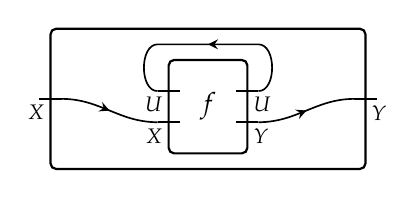
\begin{tikzpicture}[wiring diagram,bby=1.2ex]
   \node[bb={2}{2}] (domain) {$f$};
   \node[bb={1}{1}, fit={(domain) ($(domain.north)+(0,1)$)}] (codomain) {};
   \draw[ar] (codomain_in1') to (domain_in2);
   \draw[ar] (domain_out2) to (codomain_out1');
   \draw[ar] let \p1=(domain.north east), \p2=(domain.north west), \n1={\y1+\bby}, \n2=\bbportlen in
      (domain_out1) to[in=0] (\x1+\n2,\n1) -- (\x2-\n2,\n1) to[out=180] (domain_in1);
   \draw[label]
       node[below left=of codomain_in1]     {$X$}
       node[below right=of codomain_out1]    {$Y$}
       node[below left=of domain_in1]     {$U$}
       node[below left=of domain_in2]     {$X$}
       node[below right=of domain_out2]    {$Y$}
       node[below right=of domain_out1]   {$U$};
\end{tikzpicture}
$$
This can be recognized as a cobordism between oriented 0-manifolds, as we discussed in
Section~\ref{sec:wds_and_cob}. Each of the six axioms is vacuous from this perspective, in
the sense that both sides of the equation correspond to the same cobordism (up to diffeomorphism). For example, here are
the axioms of \emph{dinaturality} and \emph{superposition}:
\begin{itemize}
   \item For every $f\colon U\otimes X\to V\otimes Y$ and $g:V\to U$ we have
      \[
         \Tr^U_{X,Y}\Big[\big(g\otimes Y\big)\circ f\Big]=\Tr^V_{X,Y}\Big[f\circ\big(g\otimes X\big)\Big];
      \]
      \[\tikzset{bbx=1cm}
         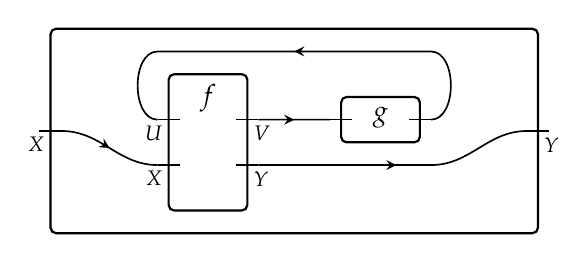
\begin{tikzpicture}[wiring diagram,baseline=(current bounding box.center)]
            \node[bb={2}{2}, bb name=$f$] (X1) {};
            \node[bb port sep=1,bb={1}{1}, right=.7 of X1_out1, bb name=$g$] (X2) {};
            \node[bb={1}{1}, fit={(X1) (X2) ($(X1.north)+(0,1)$)}] (Y) {};
            \draw[ar] (Y_in1') to (X1_in2);
            \draw[ar,pos=.8] (X1_out1) to (X2_in1);
            \draw[ar] let \p1=(X2.south east), \n1={\y1-\bby}, \n2=\bbportlen in
                (X1_out2) -- (\x1+\n2,\n1) to (Y_out1');
            \draw[ar] let \p1=(X2.north east), \p2=(X1.north west), \n1={\y2+\bby}, \n2=\bbportlen in
                  (X2_out1) to[in=0] (\x1+\n2,\n1) -- (\x2-\n2,\n1) to[out=180] (X1_in1);
            \draw[label]
                node[below left=of Y_in1]     {$X$}
                node[below right=of Y_out1]    {$Y$}
                node[below left=of X1_in1]     {$U$}
                node[below left=of X1_in2]     {$X$}
                node[below right=of X1_out2]    {$Y$}
                node[below right=of X1_out1]   {$V$};
         \end{tikzpicture}
         \quad=\quad
         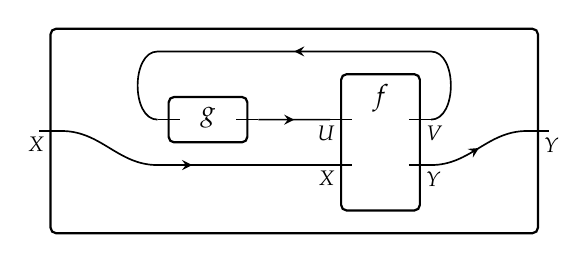
\begin{tikzpicture}[wiring diagram,baseline=(current bounding box.center)]
            \node[bb={2}{2}, bb name=$f$] (X1) {};
            \node[bb port sep=1,bb={1}{1}, left=.7 of X1_in1, bb name=$g$] (X2) {};
            \node[bb={1}{1}, fit={(X1) (X2) ($(X1.north)+(0,1)$)}] (Y) {};
            \draw[ar] let \p1=(X2.south west), \n1={\y1-\bby}, \n2=\bbportlen in
                (Y_in1') to (\x1-\n2,\n1) -- (X1_in2);
            \draw[ar] (X2_out1) to (X1_in1);
            \draw[ar] (X1_out2) to (Y_out1');
            \draw[ar] let \p1=(X1.north east), \p2=(X2.north west), \n1={\y1+\bby}, \n2=\bbportlen in
                  (X1_out1) to[in=0] (\x1+\n2,\n1) -- (\x2-\n2,\n1) to[out=180] (X2_in1);
            \draw[label]
                node[below left=of Y_in1]     {$X$}
                node[below right=of Y_out1]    {$Y$}
                node[below left=of X1_in1]     {$U$}
                node[below left=of X1_in2]     {$X$}
                node[below right=of X1_out2]    {$Y$}
                node[below right=of X1_out1]   {$V$};
         \end{tikzpicture}
         \]
   \item For every $f\colon U\otimes X\to U\otimes Y$ and $g\colon W\to Z$ we have
      \[
         \Tr^U_{X,Y}\big[f\big]\otimes g=\Tr^U_{X\otimes W,Y\otimes Z}\big[f\otimes g\big];
      \]
      \[\tikzset{bbx=.8cm,bb port sep=1.5}
      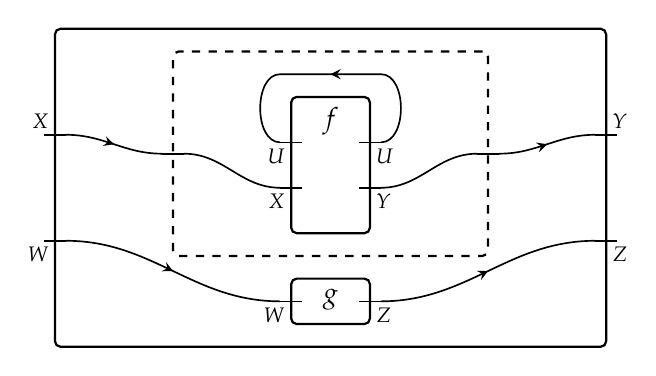
\begin{tikzpicture}[wiring diagram,baseline=(current bounding box.center)]
         \node[bb={2}{2}, bb name=$f$] (X1) {};
         \node[bb port sep=1,bb={1}{1}, below=2 of X1, bb name=$g$] (X2) {};
         \node[bb={1}{1}, fit={(X1) ($(X1.north)+(0,1)$)}, dashed] (Z) {};
         \node[bb={2}{2}, fit={(Z) (X2)}] (Y) {};
         \draw[ar] (Y_in1') to (Z_in1);
         \draw (Z_in1') to (X1_in2);
         \draw[ar] (Y_in2') to (X2_in1);
         \draw (X1_out2) to (Z_out1');
         \draw[ar] (Z_out1) to (Y_out1');
         \draw[ar] (X2_out1) to (Y_out2');
         \draw[ar] let \p1=(X1.north east), \p2=(X2.north west), \n1={\y1+\bby}, \n2=\bbportlen in
             (X1_out1) to[in=0] (\x1+\n2,\n1) -- (\x2-\n2,\n1) to[out=180] (X1_in1);
         \draw[label]
             node[above left=of Y_in1] {$X$}
             node[below left=of Y_in2] {$W$}
             node[above right=of Y_out1] {$Y$}
             node[below right=of Y_out2] {$Z$}
             node[below left=of X1_in1] {$U$}
             node[below left=of X1_in2] {$X$}
             node[below right=of X1_out2] {$Y$}
             node[below right=of X1_out1] {$U$}
             node[below left=of X2_in1] {$W$}
             node[below right=of X2_out1] {$Z$};
      \end{tikzpicture}
      \quad=\quad
      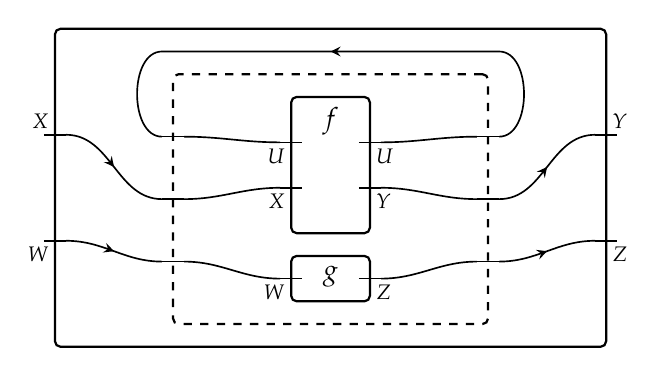
\begin{tikzpicture}[wiring diagram,baseline=(current bounding box.center)]
         \node[bb={2}{2}, bb name=$f$] (X1) {};
         \node[bb port sep=1,bb={1}{1}, below=of X1, bb name=$g$] (X2) {};
         \node[bb={3}{3}, fit={(X1) (X2)}, dashed] (Z) {};
         \node[bb={2}{2}, fit={(Z) ($(Z.north)+(0,1)$)}] (Y) {};
         \draw[ar] (Y_in1') to (Z_in2);
         \draw (Z_in2') to (X1_in2);
         \draw[ar] (Y_in2') to (Z_in3);
         \draw (Z_in3') to (X2_in1);
         \draw (X1_out2) to (Z_out2');
         \draw[ar] (Z_out2) to (Y_out1');
         \draw (X2_out1) to (Z_out3');
         \draw[ar] (Z_out3) to (Y_out2');
         \draw (Z_in1') to (X1_in1);
         \draw (X1_out1) to (Z_out1');
         \draw[ar] let \p1=(Z.north east), \p2=(Z.north west), \n1={\y1+\bby}, \n2=\bbportlen in
             (Z_out1) to[in=0] (\x1+\n2,\n1) -- (\x2-\n2,\n1) to[out=180] (Z_in1);
         \draw[label]
             node[above left=of Y_in1] {$X$}
             node[below left=of Y_in2] {$W$}
             node[above right=of Y_out1] {$Y$}
             node[below right=of Y_out2] {$Z$}
             node[below left=of X1_in1] {$U$}
             node[below left=of X1_in2] {$X$}
             node[below right=of X1_out2] {$Y$}
             node[below right=of X1_out1] {$U$}
             node[below left=of X2_in1] {$W$}
             node[below right=of X2_out1] {$Z$};
      \end{tikzpicture}
      \]
\end{itemize}

The definition of traced categories and traced functors can be found in~\cite{JoyalStreetVerity}. However, those authors define the 2-morphisms between traced functors to be monoidal transformations, whereas this choice does not behave appropriately with their $\Int$ construction (for example $\Int$ would not be 2-functorial). A correction was made in \cite{HK}, where it was shown that the appropriate 2-morphisms between traced functors are natural \emph{isomorphisms}. We denote by $\TTrCat$ the corrected 2-category of traced categories (where 2-cells are invertible), and we denote its underlying 1-category by $\TrCat$.

%\subsection{The categories $\Prop$ and $\TrProp$ of props and traced props}\label{sec:defining props}
%\todo{Do we want to use this section anywhere?}
%
%One can think of a prop as a symmetric monoidal category whose objects are free on a fixed set of \emph{labels}
%(also known as its set of colors). Functors between props need to descend to a function between
%label sets. We define a traced prop to be a traced category whose underlying symmetric monoidal
%category has the structure of a prop. Thus we have defined the 1-categories $\Prop$ and $\TrProp$;
%we summarize our definitions by the pullback diagram of categories
%\[
%\begin{tikzcd}
%   \TrProp\ar[r]\ar[d]\arrow[dr, phantom, "\lrcorner", very near start]&\TrCat\ar[d]\\
%   \Prop\ar[r]\ar[d,"\tn{Labels}"']\arrow[dr, phantom, "\lrcorner", very near start]&\MonCat\ar[d,"\Ob"]\\
%   \Set\ar[r,"\TM"']&\Set
%\end{tikzcd}
%\]
%where $\TM\colon\Set\to\Set$ is the free monoid monad. This definition of $\Prop$
%agrees with that in~\cite{HackneyRobertson}.\todo{Check this.}
%

\section{Compact categories and the Int construction}\label{sec:compact_and_int}

We will denote by $\CCompCat$ the full sub-2-category of $\MMonCat$ spanned by the compact symmetric
monoidal categories (or just compact categories for short).  Recall that a compact category is a
symmetric monoidal category $(\cat{C},\otimes,I)$ with the property that for every object
$X\in\Ob\cat{C}$ there exists an object $X^*$ and morphisms $\eta_X\colon I\to X^*\otimes X$ and
$\epsilon_X\colon X\otimes X^*\to I$ such that the following diagrams commute:
\begin{equation*}
   \begin{tikzcd}[column sep=small]
      X\arrow[r,"\id_X"]\arrow[d,"\cong"'] & X \\
      X\otimes I\arrow[d,"X\otimes\eta_X"'] & I\otimes X\arrow[u,"\cong"'] \\
      X\otimes(X^*\otimes X)\arrow[r,"\cong"'] & (X\otimes X^*)\otimes X\arrow[u,"\epsilon_X\otimes X"']
   \end{tikzcd}
   \hspace{.6in}
   \begin{tikzcd}[column sep=small]
      X^*\arrow[r,"\id_{X^*}"]\arrow[d,"\cong"'] & X^*\\
      I\otimes X^*\arrow[d,"\eta_X\otimes X^*"'] & X^*\otimes I\arrow[u,"\cong"'] \\
      (X^*\otimes X)\otimes X^*\arrow[r,"\cong"'] & X^*\otimes (X\otimes X^*)\arrow[u,"X^*\otimes\epsilon_X"']
   \end{tikzcd}
\end{equation*}

Every compact category $\cat{C}$ has a canonical trace structure, defined on a morphism $f\colon
U\otimes X\to U\otimes Y$ to morally be $\epsilon_U\circ f\circ \eta_U$. More precisely, if
$\sigma_{A,B}$ is the symmetry isomorphism, one defines
\begin{equation*}
   \Tr^U_{X,Y}[f]\coloneqq(\epsilon_U\otimes Y)\circ (\sigma_{U^*,U}\otimes Y)\circ (U^*\otimes f)\circ (\eta_U\otimes X)
\end{equation*}
%\todo[color=yellow]{does this formula make sense as written? i.e. it doesn't seem to give a map
%$X\to Y$?}
Thus we have a functor $\UCT\colon\CCompCat\to\TTrCat$. It is shown in~\cite{JoyalStreetVerity}~and~\cite{HK} that
this functor is the right half of a 2-adjunction
\begin{equation}\label{dia:traced_compact_adjunction}
\begin{tikzcd}
   \TTrCat\arrow[r,shift left=.5ex, "\Int"]&\CCompCat\arrow[l,shift left=.5ex,"\UCT"]
\end{tikzcd}
\end{equation}
the left half of which we now describe on the level of objects $\cat{M}\in\Ob\TTrCat$.

For a traced category $\cat{M}$, let $\widetilde{\cat{M}}$ denote the category with
objects given by pairs $(\inp{X},\outp{X})$ where $\inp{X},\outp{X}\in \Ob(\cat{M})$ and morphisms
given by
\[
   \Hom_{\widetilde{\cat{M}}}\big((\inp{X},\outp{X}),(\inp{Y},\outp{Y})\big)=\Hom_{\cat{M}}(\inp{X}\otimes \outp{Y},\outp{X}\otimes \inp{Y}).
\]
For morphisms $\Phi:(\inp{X},\outp{X})\to(\inp{Y},\outp{Y})$ and $\Psi:(\inp{Y},\outp{Y})\to(\inp{Z},\outp{Z})$ in $\widetilde{\cat{M}}$ we define their composition to be
\[
   \Psi\circ\Phi\coloneqq\Tr^{\outp{Y}}_{\inp{X}\otimes \outp{Z},\outp{X}\otimes \inp{Z}}\Big[\big(\gamma_{\outp{X},\outp{Y}}\otimes \inp{Z}\big)\circ\big(\outp{X}\otimes\Psi\big)\circ\big(\Phi\otimes \outp{Z}\big)\circ\big(\gamma_{\outp{Y},\inp{X}}\otimes \outp{Z}\big)\Big].
\]
It is shown in~\cite{JoyalStreetVerity} that $\Int(\cat{M})\coloneqq\widetilde{\cat{M}}$ is a compact category whose tensor is given by
\[
   (\inp{X},\outp{X})\odot(\inp{Y},\outp{Y})\coloneqq(\inp{X}\otimes \inp{Y},\outp{X}\otimes \outp{Y})
\]
with unit object $\tilde I\coloneqq(I,I)$ and duality ${(\inp{X},\outp{X})}^\vee\coloneqq(\outp{X},\inp{X})$.

%The following is immediate from the definitions above and in Section~\ref{sec:scalars and elements}.

%\todo{Do we use Lemma~\ref{lemma:elements in traced}? Does it give intuition?}
%\begin{lemma}\label{lemma:elements in traced}\todo{This lemma has a sign-error. Either change definition of $\Hom_{\widetilde{\cat{M}}}$ or lemma statement.}
%
%Let $\cat{M}$ be a traced category and $\widetilde{\cat{M}}=Int(\cat{M})$ its compact closure. If $|\cdot|$ is the elements algebra on $\widetilde{\cat{M}}$, then for any object $(\inp{X},\outp{X})\in\Ob\widetilde{\cat{M}}$ there is a canonical bijection
%\[|(\inp{X},\outp{X})|\iso\Hom_{\cat{M}}(\inp{X},\outp{X}).\]
%
%\end{lemma}
%

\begin{lemma}\label{lemma:fully_faithful_and_trace}
The following facts hold for any traced category $\cat{C}$:
\begin{compactenum}[\quad i.]
   \item The unit $\cat{C}\to\Int(\cat{C})$ is fully faithful.
   \item If $\cat{D}$ is a category and $F\colon\cat{D}\to\cat{C}$ a fully faithful symmetric
      monoidal functor, then $\cat{D}$ has a unique trace for which $F$ is a traced functor.
   \item If $\cat{C}$ is compact then the unit $\cat{C}\To{\equiv}\Int(\cat{C})$ is an equivalence.
   \item Suppose that $\cat{C'}$ is a traced category and that $F\colon \cat{C}\to \cat{C}'$ is a
      traced functor. Then $F$ is bijective-on-objects (resp. fully faithful) if and only if
      $\Int(F)$ is.
\end{compactenum}
\end{lemma}
\begin{proof}
   These are all shown in, or trivially derived from,~\cite{JoyalStreetVerity}.
\end{proof}

\section{Free traced and compact categories, and geometry}\label{sec:free_and_geometry}

There are free/forgetful adjunctions
\begin{align*}
   \FM\colon\Set &\leftrightarrows\MonCat:\!\UM \\
   \FT\colon\Set &\leftrightarrows\TrCat:\!\UT \\
   \FC\colon\Set &\leftrightarrows\CompCat:\!\UC
\end{align*}
We will write $\TM, \TT$, and $\TC$ for the respective monads induced on $\Set$. Note that $\TM$ is
isomorphic to the free-monoid monad, while $\TC$ is isomorphic to the free-group monad.%
\footnote{Note that $U_M$ is not the free-\emph{commutative}-monoid monad, even though the objects of $\MonCat$ are \emph{symmetric} monoidal categories, because the symmetries are encoded in natural isomorphisms, not equalities.
}
We will denote by $\FrMonCat$ and $\FrCompCat$ the full subcategories of $\MonCat$ and $\CompCat$
respectively, spanned by objects which are free on a set. As always, these categories are isomorphic
to the Kleisli categories of the monads: 
\begin{align}\label{dia:TMvsFrMonCat}
\FrMonCat&\iso\Set_{\TM}
\\\nonumber
\FrCompCat&\iso\Set_{\TC}.
\end{align}

The forgetful functors between the categories of structured monoidal categories commute with the
underlying set functors, i.e.~the following diagram commutes:
%\begin{equation*}
%	\begin{tikzcd}[column sep=large]
%	\CompCat\ar[r,"\UCT"]\ar[rd,"\UC"']\ar[rr,bend left,"\UCM"]&\TrCat\ar[r,"\UTM"]\ar[d,"\UT"]&\MonCat\ar[dl,"\UM"]\\
%	&\Set
%	\end{tikzcd}
%\end{equation*}

\begin{equation*}
   \begin{tikzcd}
      & \TrCat \ar[dr,"\UTM"] \ar[dd,"\UT" near start] & \\
      \CompCat \ar[rr,crossing over,"\UCM"' near start] \ar[dr,"\UC"'] \ar[ru,"\UCT"]
         && \MonCat \ar[dl,"\UM"] \\
      & \Set &
   \end{tikzcd}
\end{equation*}
Because the functor $\UCM\colon\CompCat\to\MonCat$ commutes with the right adjoints of the
adjunctions to $\Set$, i.e., $\UM\UCM=\UC$, it induces a monad morphism $\alpha\colon\TC\to\TM$ (a natural transformation
$\alpha\colon\TM\to\TC$ compatible with the units and multipications), given by the composition of
the natural transformations
%\begin{equation*}
%   \begin{tikzcd}[column sep=large,row sep=0ex]
%      \TM=\UM\FM \ar[r,"\UM\FM\eta_C"]
%         & \UM\FM\UC\FC = \UM\FM\UM\UCM\FC \\
%      \UM\FM\UM\UCM\FC \ar[r,"\UM\epsilon_M\UCM\FC"']
%         & \UM\UCM\FC = \UC\FC = \TC
%   \end{tikzcd}
%\end{equation*}
\begin{equation*}
	\begin{tikzcd}[column sep=2cm]
		\TM\ar[r,equal]\ar[d,dashed,"\alpha"']&\UM\FM\ar[r,"\UM\FM\eta_C"]&\UM\FM\UC\FC\ar[d,equal]\\
		\TC&\UM\UCM\FC\ar[l,equal]&\UM\FM\UM\UCM\FC\ar[l,"\UM\epsilon_M\UCM\FC"]
	\end{tikzcd}
\end{equation*}
The components $\alpha_{\LabSet}$ of this transformation are simply the evident inclusion of the free monoid on a set
$\LabSet$ into the free group on $\LabSet$. In this way, $\UCM$ induces a functor between the Kleisli categories in the other direction:
\begin{equation}\label{eqn:FMC}
   \FMC\colon\FrMonCat\to\FrCompCat
\end{equation}

%\begin{proposition}\label{prop:free traced and compact}
%   Let $\cat{C}$ be a category.
%   The free traced category on $\cat{C}$ is...
%   The free compact category on $\cat{C}$ is $\Int(...)$.\todo{Fill this in}
%\end{proposition}
%\begin{proof}
%   Kelly, Laplaza ``Coherence for compact closed categories'' gives a combinatorial description of
%   the free compact category on one object.
%
%   See Abramsky.
%\end{proof}

\subsection{$\LCob{\LabSet}$ is the free compact category on $\LabSet$}

To connect the geometry (string diagrams) with the algebra (free compact categories), we recall the following folklore theorem. 

\begin{theorem}
The free compact category on one generator is equivalent to $\Cob$, the category of oriented 1-dimensional cobordisms.
\end{theorem}

See \cite[Theorem 3.6]{FreydYetter} for a proof of the non-symmetric version, \cite{Kock} and \cite{BaezDolan} for the 2-dimensional version with brief comments on the 1-dimensional version. See also \cite{KellyLaplaza} and \cite{Abramsky2} for combinatorial descriptions of $\Cob$ as the free compact category functor.  Because the free functor is a left adjoint, we have the following corollary.

\begin{corollary}\label{cor:free_compact_is_Cob}

For any set $\LabSet$, the free compact category on $\LabSet$ is equivalent to $\LCob{O}$, the category of oriented $\LabSet$-labeled 1-cobordisms. 

\end{corollary}

%   Joachim Kock proves that 2-cob is the free compact category on a frobenius algebra object, and
%   the proof can be adapted.

\section{Orthogonal factorization systems}

We use orthogonal factorization systems throughout this paper, mainly to deal with the issue of object-variance, mentioned in Section~\ref{subsec:main_results}. Background on orthogonal factorization systems can be found in \cite[Chapter 5.5]{BorceuxV1}. Here we describe the $\cat{V}$-enriched notion, for two cases, the usual 1-categorical case, where $\cat{V}=\Set$, and the strict 2-categorical case, where $\cat{V}=\Cat$.

\begin{definition}\label{def:orthogonal}
Let $\cat{V}$ be either $\Set$ or $\Cat$, and suppose that $\cat{C}$ is a $\cat{V}$-enriched category. A \emph{orthogonal factorization system in $\cat{C}$} consists of two distinguished classes of morphisms, $(\cat{L},\cat{R})$ with the following properties:
\begin{itemize}
\item each morphism $f\in\cat{C}$ factors as $f=e\circ m$, where $m\in\cat{L}$ and $e\in\cat{R}$;
\item if $m\colon a\to b$ in $\cat{L}$ and $e\colon c\to d$ in $\cat{R}$, then the left-hand square below is a pullback in $\cat{V}$:
\begin{equation}\label{eqn:OrthFactSys}
\begin{tikzcd}
\cat{C}(b,c)\ar[r]\ar[d]\ar[rd,phantom,"\lrcorner" very near start]&\cat{C}(a,c)\ar[d,"e\circ -"]\\
\cat{C}(b,d)\ar[r,"-\circ m"']&\cat{C}(a,d)
\end{tikzcd}
\hspace{.9in}
\begin{tikzcd}
a\ar[r,"\forall"]\ar[d,two heads,"m"']&c\ar[d,hook, "e"]\\
b\ar[r,"\forall"']\ar[ur,dashed,"\exists!"]&d
\end{tikzcd}
\end{equation}
In particular, for all solid arrow squares, as in the right-hand diagram, there exists a unique diagonal filler. 
\end{itemize}
As shown, we often indicate morphisms in $\cat{L}$ using a two-headed arrow, and morphisms in $\cat{R}$ using a hooked arrow.
\end{definition}

If $\ccat{C}$ is a 2-category and $\cat{L}, \cat{R}$ are distinguished classes of morphisms, we say that $\cat{L}$ is \emph{left pseudo-orthogonal} to $\cat{R}$ if the pullback square (left of \eqref{eqn:OrthFactSys}) is only required to be a pseudo-pullback. This means that for any pseudo-commuting square (right of \eqref{eqn:OrthFactSys}), there exists an essentially unique pseudo-commuting lift.

\begin{example}\label{ex:ess_surj_pseudo_ff}
In $\CCat$, the class of essentially surjective functors is left pseudo-orthogonal to the class of fully faithful functors.
\end{example}

\begin{remark}

As in Definition~\ref{def:orthogonal}, we will use the hooked arrow $\inj$ to indicate $\ff$ morphisms and the two-headed arrow $\tto$ to indicate $\bo$ morphisms. However, we sometimes use the latter symbol to indicate fibrations of categories (e.g., as we did in \ref{thm:TheoremB}). These two uses of the symbol $\tto$ can be distinguished as follows. If the arrow occurs between objects in an equipment, then it indicates a $\bo$ map; if it occurs as a structural part of a given equipment, e.g., as in Definition~\ref{def:equipment}, then it indicates a fibration. 

\end{remark}

\chapter{Background on equipments}\label{sec:background_equipments}

\section{Motivating example: manipulating profunctors}
Let $\cat{C}$ and $\cat{D}$ be categories.
Recall that a profunctor $M$ from $\cat{C}$ to $\cat{D}$, written
\[
\begin{tikzcd}
   \cat{C} \ar[r,tick,"M"] & \cat{D},
\end{tikzcd}
\]
is defined to be a functor $M\colon\op{\cat{C}}\times\cat{D}\to\Set$. We can think of a profunctor
as a sort of graded bimodule: for each object $c\in\cat{C}$ and $d\in\cat{D}$ there is a set
$M(c,d)$ of elements in the bimodule, and given an element $m\in M(c,d)$ and morphisms $f\colon
c'\to c$ in $\cat{C}$ and $g\colon d\to d'$ in $\cat{D}$, there are elements $g\cdot m\in M(c,d')$
and $m\cdot f\in F(c',d)$, such that $(g\cdot m)\cdot f=g\cdot(m\cdot f)$, and $g'\cdot(g\cdot
m)=(g'\circ g)\cdot m$ and $(m\cdot f)\cdot f'=m\cdot(f\circ f')$ whenever they make sense.

If $F\colon\cat{C}'\to\cat{C}$ and $G\colon\cat{D}'\to\cat{D}$ are functors, and $M$ is a profunctor
as before, then there is a profunctor $M(F,G)$ from $\cat{C}'$ to $\cat{D}'$, defined to be the
composite
\[
\begin{tikzcd}
   \op{\cat{C}'}\times\cat{D}' \ar[r,"\op{F}\times G"]
      &[1.5em] \op{\cat{C}}\times\cat{D} \ar[r,"M"]
      & \Set.
\end{tikzcd}
\]
In other words, for any objects $c\in\cat{C}'$ and $d\in\cat{D}'$, the profunctor $M(F,G)$ has
elements $M(Fc,Gd)$, and if $m\in M(Fc,Gd)$ and $g\colon d\to d'$ is a morphism in $\cat{D}'$, then
the element $m\cdot g$ in $M(F,G)$ is defined by the element $m\cdot G(g)$ in $M$, and similarly for
the $\cat{C}'$ action.

Given two profunctors
\[
\begin{tikzcd}
   \cat{C} \ar[r,tick,shift left,"M"] \ar[r,tick,shift right,"N"'] & \cat{D}
\end{tikzcd}
\]
define a profunctor morphism $\phi\colon M\Rightarrow N$ to be a natural transformation. In other
words, for each $c\in\cat{C}$ and $d\in\cat{D}$ there is a function $\phi_{c,d}\colon M(c,d)\to
N(c,d)$ such that $\phi(f\cdot m \cdot g)=f\cdot\phi(m)\cdot g$ whenever it makes sense.

There is a tensor product of profunctors: given two profunctors
\[
\begin{tikzcd}
   \cat{C} \ar[r,tick,"M"] & \cat{D} \ar[r,tick,"N"] & \cat{E}
\end{tikzcd}
\]
define the profunctor $M\otimes N$ such that for objects $c\in\cat{C}$ and $e\in\cat{E}$, $(M\otimes
N)(c,e)$ is the coequalizer of the diagram
\[
\begin{tikzcd}
   \displaystyle\coprod_{d_1,d_2\in\cat{D}} M(c,d_1)\times\cat{D}(d_1,d_2)\times N(d_2,e)
      \ar[r,shift left] \ar[r,shift right]
   & \displaystyle\coprod_{d\in\cat{D}} M(c,d)\times N(d,e)
\end{tikzcd}
\]
where the two maps are given by the right action of $\cat{D}$ on $M$ and by the left action of
$\cat{D}$ on $N$. We can write elements of $(M\otimes N)(c,e)$ as tensors $m\otimes n$, where $m\in
M(c,d)$ and $n\in N(d,e)$ for some $d\in\cat{D}$. The coequalizer then implies that $(m\cdot
f)\otimes n=m\otimes(f\cdot n)$ whenever the equation makes sense.

For any category $\cat{C}$, there is a profunctor
$\Hom_{\cat{C}}\colon\op{\cat{C}}\times\cat{C}\to\Set$, and these hom profunctors act as units for
the tensor product. Precisely, if $M$ is as above, there are canonical isomorphisms
$\Hom_{\cat{C}}\otimes M \iso M \iso M\otimes\Hom_{\cat{D}}$.

\section{Equipments}

A double category is a 2-category-like structure involving horizontal and vertical arrows, as well as 2-cells. An equipment (sometimes called a \emph{proarrow equipment} or \emph{framed bicategory}) is a double category satisfying a certain fibrancy condition. In this section, we will spell this out and give a few examples. An excellent reference is Shulman's paper \cite{Shulman}.

\begin{definition}
   A \emph{double category} $\dcat{D}$ consists of the following data:
   \begin{compactitem}
      \item A category $\dcat{D}_0$, which we refer to as the \emph{vertical category} of
         $\dcat{D}$. For any two objects $c,d\in\dcat{D}_0$, we will write
         $\dcat{D}(c,d)=\dcat{D}_0(c,d)$ for the set of vertical arrows from $c$ to $d$. We refer to
         objects of $\dcat{D}_0$ as objects of $\dcat{D}$.
      \item A category $\dcat{D}_1$, equipped with two functors $L,R\colon\dcat{D}_1\to\dcat{D}_0$,
         called the \emph{left frame} and \emph{right frame} functors. Given an object
         $A\in\Ob\dcat{D}_1$ with $c=L(A)$ and $c'=R(A)$, we say that $A$ is a \emph{proarrow} (or
            \emph{horizontal arrow}) \emph{from $c$ to $c'$} and write $A\colon c\tickar c'$. A
            morphism $\phi\colon A\to B$ in $\dcat{D}_1$ is called a 2-cell, and is drawn as
            follows, where $f=L(\phi)$ and $f'=R(\phi)$:
         \begin{equation*}
            \begin{tikzcd}
               c \ar[r,tick,"A" domA] \ar[d,"f"']
               & c'\ar[d,"{f'}"]
                 \\
               d \ar[r,tick,"B"' codA]
                 & d'
               \twocellA{\phi}
            \end{tikzcd}
         \end{equation*}
      \item A \emph{unit} functor $U\colon\dcat{D}_0\to\dcat{D}_1$, which is a
         retraction of both $L$ and $R$, i.e., $L\circ U=\id_{\dcat{D}_0}=R\circ U$. We will often
         abuse notation by writing $c$ for the unit proarrow $U(c)\colon c\tickar c$, and similarly
         for vertical arrows.
      \item A functor $\odot\colon\dcat{D}_1\times_{\dcat{D}_0}\dcat{D}_1\to\dcat{D}_1$, called
         \emph{horizontal composition}, that is weakly associative and unital in the sense that
         there are coherent unitor and associator isomorphisms. See \cite{Shulman} for details.
   \end{compactitem}
   Given a double category $\dcat{D}$ there is a strict 2-category called the \emph{vertical
   2-category}, denoted $\VVer(\dcat{D})$, whose underlying 1-category is $\dcat{D}_0$, and whose
   2-morphisms are given by $\VVer(\dcat{D})(f,g)\coloneqq\dcat{D}_1(Uf,Ug)$. There is also a
   \emph{horizontal bicategory}, denoted $\HHor(\dcat{D})$, obtained from $\dcat{D}$ by requiring
   $F=\id_A, G=\id_B$; see Example~\ref{ex:horizontal_bicategory}.
   
   A \emph{strong double functor} $\dcat{D}\to\dcat{E}$ consists of functors $\dcat{D}_0\to\dcat{E}_0$ and
   $\dcat{D}_1\to\dcat{E}_1$ commuting with the frames $L,R$, and preserving the unit $U$ and
   horizontal composition $\odot$ up to coherent isomorphism. There is also a notion of \emph{lax
   double functor} which only preserves units and composition up to non-invertible 2-cell. While
   important to the theory of double categories and equipments in general, in this paper we will
   only be concerned with strong double functors.
\end{definition}

\begin{definition}\label{def:equipment}
   An \emph{equipment} is a double category $\dcat{D}$ in which the functor
   \begin{equation*}
      (L,R)\colon\dcat{D}_1\tto\dcat{D}_0\times\dcat{D}_0
   \end{equation*}
   is a fibration. If $f\colon c\to c'$ and $g\colon d\to d'$ are vertical morphisms and $B\colon
   c'\tickar d'$ is a proarrow, a cartesian morphism $A\to B$ in $\dcat{D}_1$ over $(f,g)$ is a
   2-cell
   \begin{equation*}
      \begin{tikzcd}
         c \ar[r,tick, "A" domA] \ar[d,"f"']
            & d\ar[d,"{g}"] \\
         c' \ar[r,tick,"B"' codA]
            & d'
         \twocellA{\tn{cart}}
      \end{tikzcd}
   \end{equation*}
   which we call a \emph{cartesian 2-cell}. We refer to $A$ as the \emph{restriction of $B$ along
   $(f,g)$}, written $B(g,f)$.

   By an \emph{equipment functor}, we simply mean a strong double functor between equipments.
\end{definition}

\begin{example}
   An equipment $\dcat{D}$ is often named according to its horizontal arrows. In
   Section~\ref{sec:background_equipments} we discussed profunctors, which are the horizontal arrows
   in an equipment $\dProf$, which we will now discuss. Variations on $\dProf$, such as $\dMonProf,
   \dTrProf,$ and $\dCompProf$ (defined in Section~\ref{sec:monoidal_profunctors}) will play a major
   role in this paper.

   The vertical category of $\dProf$ is the 1-category $\dProf_0=\Cat$ of small 1-categories and
   functors. Given objects $C,D\in\dProf_0$, a horizontal arrow between them is a profunctor
   $C\tickar D$, as described in Section~\ref{sec:background_equipments}. A 2-cell $\phi$ in
   $\dProf$, as to the left, denotes a natural transformation, as to the right, in
   \eqref{eqn:Prof2cells}:
   \begin{equation}\label{eqn:Prof2cells}
      \begin{tikzcd}
         A \ar[r,tick,"X" domA] \ar[d,"F"']
            & B\ar[d,"{G}"] \\
         C \ar[r,tick,"Y"' codA]
            & D
         \twocellA{\phi}
      \end{tikzcd}
      \hspace{.6in}
      \begin{tikzcd}[column sep=.8em, row sep=5ex]
         \op{A}\times B \ar[dr,"X"'] \ar[rr,"\op{F}\times G"]
            & \ar[d,phantom,"\overset{\phi}{\Rightarrow}" near start]
            & \op{C}\times D\ar[dl,"Y"] \\
         & \Set
      \end{tikzcd}
   \end{equation}
   The horizontal composite $X\odot Y$ of profunctors $X\colon A\tickar B$ and $Y\colon B\tickar C$
   is obtained by a coend formula, equivalent to the following coequalizer for any $a\in\op{A}, c\in
   C$:
   \begin{equation}\label{eqn:coendComp}
      \begin{tikzcd}
         \displaystyle\coprod_{b_1,b_2}X(a,b_1)\times\ B(b_1,b_2)\times Y(b_2,c)
               \ar[r,shift left,"b=b_1"]\ar[r,shift right,"b=b_2"']
            & \displaystyle\coprod_{b}X(a,b)\times Y(b,c) \ar[r]
            &[-1em] (X\odot Y)(a,c)
      \end{tikzcd}
   \end{equation}
   One can show that the result is a double category, and it is an equipment because for any $F,
   G,Y$ as in \eqref{eqn:Prof2cells}, there is a cartesian 2-cell whose domain is the profunctor
   $X=Y\circ(\op{F}\times G)$ obtained by composition.

   Note that the coequalizer \eqref{eqn:coendComp} is in fact a reflexive coequalizer, using
   $f=\id_b$.
\end{example}

\begin{example}\label{ex:dspan}
   There is an equipment $\dSpan$ of spans in $\Set$. Its vertical category is
   $\dSpan_0\coloneqq\Set$. A horizontal 1-cell between sets $A$ and $B$ is a span $A\from S\to B$,
   their composition is defined by a pullback of spans, and a 2-cell in $\dSpan$ is a commutative
   diagram in $\Set$ of the obvious shape. The cartesian 2-cells in this equipment are obtained by
   taking a limit in $\Set$.
\end{example}

\begin{definition}\label{def:local_equivalence}
   An equipment functor $F\colon\dcat{X}\to\dcat{Y}$ is a \emph{local equivalence} if the following
   square is a pseudo-pullback of categories:
   \begin{equation}\label{eqn:local_equiv}
      \begin{tikzcd}
         \dcat{X}_1 \ar[r] \ar[d,two heads] \ar[dr,phantom,"\lrcorner" very near start]
            & \dcat{Y}_1 \ar[d,two heads] \\
         \dcat{X}_0\times\dcat{X}_0 \ar[r]
            & \dcat{Y}_0\times\dcat{Y}_0
      \end{tikzcd}
   \end{equation}
   If $F_0\colon\dcat{X}_0\to\dcat{Y}_0$ is fully faithful, we say that $F$ is a \emph{fully faithful local equivalence}.
\end{definition}

\begin{remark}\label{rem:strict_vs_pseudo_pullback}
   It is a standard fact that a strict pullback of categories of an isofibration along an arbitrary
   functor is also a pseudo-pullback. As any Grothendieck fibration (or opfibration) is in
   particular an isofibration, if the square \eqref{eqn:local_equiv} is a strict pullback, then it
   is also a pseudo-pullback.
\end{remark}

\begin{definition}\label{def:induced_locally_equivalent_equipment}
   Let $\dcat{Y}$ be a double category and $F_0\colon\dcat{X}_0\to\dcat{Y}_0$ be a functor. A strict
   pullback of the form \eqref{eqn:local_equiv} defines a double category $\dcat{X}$, which we denote
   \begin{equation}
    \dcat{X}\coloneqq F_0^*(\dcat{Y})
   \end{equation} 
   and call the \emph{equipment induced by $F_0$}. If $\dcat{Y}$ is an equipment, $F_0^*(\dcat{Y})$ will be too, because fibrations are
   stable under pullback. By Remark~\ref{rem:strict_vs_pseudo_pullback}, the obvious equipment
   functor $F_0^*(\dcat{Y})\to\dcat{Y}$ is a local equivalence.
\end{definition}

\begin{example}\label{ex:horizontal_bicategory}
   The horizontal bicategory $\HHor(\dcat{D})$ associated to an equipment $\dcat{D}$ can be
   identified with the locally equivalent equipment induced by the inclusion
   $\Ob\dcat{D}_0\to\dcat{D}_0$ of the discrete category of objects. 

   It follows that if $\dcat{D}\to\dcat{E}$ is a local equivalence of equipments, then
   $\HHor(\dcat{D})\to\HHor(\dcat{E})$ is a local equivalence of bicategories. Note, however, that
   the converse does not hold in general.
\end{example}

% \begin{definition}\todo{Do we need this? Consider deleting this and Lemma~\ref{lemma:delete_me?}.}

% Let $F\colon\dcat{D}\to\dcat{E}$ be an equipment functor. We say that $F$ is \emph{fully faithful} if both $F_0$ and $F_1$ are, i.e., if both the following squares are pullbacks in $\Set$:
% $$
% 	\begin{tikzcd}[column sep=2em]
% 		\Mor\dcat{D}_0\ar[r,"\Mor F_0"]\ar[d]\ar[dr,phantom,"\lrcorner" very near start]&\Mor\dcat{E}_0\ar[d]\\
% 		\Ob\dcat{D}_0\times\Ob\dcat{D}_0\ar[r,"\Ob F_0"']&\Ob\dcat{E}_0\times\Ob\dcat{E}_0
% 	\end{tikzcd}
% \qquad
% 	\begin{tikzcd}[column sep=2em]
% 		\Mor\dcat{D}_1\ar[r,"\Mor F_1"]\ar[d]\ar[dr,phantom,"\lrcorner" very near start]&\Mor\dcat{E}_1\ar[d]\\
% 		\Ob\dcat{D}_1\times\Ob\dcat{D}_1\ar[r,"\Ob F_1"']&\Ob\dcat{E}_1\times\Ob\dcat{E}_1
% 	\end{tikzcd}
% $$

% \end{definition}

\section{The monoids and bimodules construction}

\begin{definition}\label{def:monoids_and_modules}
   Let $\dcat{D}$ be an equipment. The equipment $\dMod(\dcat{D})$ of \emph{monoids and bimodules} is
   defined as follows:
   \begin{compactitem}
      \item The objects are \emph{monoids} in $\dcat{D}$: tuples $(c,M,e_M,m_M)$ consisting of an
         object $c$ of $\dcat{D}$, a proarrow $M\colon c\tickar c$, and unit and
         multiplication cells
         \begin{equation*}
            \begin{tikzcd}
               c \ar[r,tick,"c" domA] \ar[d,equal]
                  & c \ar[d,equal] \\
               c \ar[r,tick,"M"' codA] & c
               \twocellA{e_M}
            \end{tikzcd}
            \qquad
            \begin{tikzcd}
              c \ar[r,tick,"M"] \ar[d,equal]
                 & |[alias=domA]| c \ar[r,tick,"M"]
                 & c \ar[d,equal] \\
              c \ar[rr,tick,"M"' codA]
                 && c
              \twocellA{m_M}
            \end{tikzcd}
         \end{equation*}
         satisfying the evident unit and associativity axioms. 
      \item The vertical arrows are \emph{monoid homomorphisms}: pairs $(f,\vec{f}\mspace{2mu})$ of a vertical arrow
         $f\colon c\to d$ in $\dcat{D}$ and a cell
         \begin{equation*}
            \begin{tikzcd}
               c \ar[r,tick,"M" domA] \ar[d,"f"']
                  & c \ar[d,"f"] \\
               d \ar[r,tick,"N"' codA]
                  & d
               \twocellA{\vec{f}}
            \end{tikzcd}
         \end{equation*}
         which respects the unit and multiplication cells of $M$ and $N$.
      \item The proarrows $B\colon M\tickar N$ are \emph{bimodules}: triples $(B,l_B,r_B)$
         consisting of a proarrow $B\colon c\tickar d$ in $\dcat{D}$ and cells
         \begin{equation*}
            \begin{tikzcd}
               c \ar[r,tick,"M"] \ar[d,equal]
                  & |[alias=domA]| c \ar[r,tick,"B"]
                  & d \ar[d,equal] \\
               c \ar[rr,"B"' codA]
                  && d
               \twocellA{l_B}
            \end{tikzcd}
            \qquad
            \begin{tikzcd}
               c \ar[r,tick,"B"] \ar[d,equal]
                  & |[alias=domA]| d \ar[r,tick,"N"]
                  & d \ar[d,equal] \\
               c \ar[rr,"B"' codA]
               && d
               \twocellA{r_B}
            \end{tikzcd}
         \end{equation*}
         satisfying evident monoid action axioms.
      \item The 2-cells are \emph{bimodule homomorphisms}: cells in $\dcat{D}$
         \begin{equation*}
            \begin{tikzcd}
              c \ar[r,tick,"A"] \ar[d,"f"' domA]
                 & d \ar[d,"g" codA] \\
              c' \ar[r,tick,"B"']
                 & d'
              \twocellA{\phi}
            \end{tikzcd}
         \end{equation*}
         which are compatible with the left and right actions of the bimodules.
   \end{compactitem}
\end{definition}

\begin{example}\label{ex:monoid_in_Prof}
   Consider a monoid $M\colon C\tickar C$ in $\dProf$. The unit is a profunctor morphism
   $i\colon\Hom_{C}\to M$. So for any $f\colon c\to d$ in $C$ there is an element
   $i(f)\in M(c,d)$, such that $f\cdot i(g)\cdot h = i(f\circ g\circ h)$ whenever this makes sense.
   The multiplication $M\otimes M\to M$ is an operation assigning to any elements $m_1\in M(c,d)$ and
   $m_2\in M(d,e)$ an element $m_2\bullet m_1\in M(c,e)$, which is associative, and satisfies the
   following equations whenever they make sense:
   \begin{gather*}
      (f\cdot m_2)\bullet(m_1\cdot h) = f\cdot(m_2\bullet m_1)\cdot h
      \\ (m_3\cdot g)\bullet m_1 = m_3\bullet(g\cdot m_1)
      \\ m\bullet i(f) = m\cdot f
            \quad\text{and}\quad
         i(g)\bullet m = g\cdot m
   \end{gather*}
\end{example}

\begin{example}\label{ex:mod_span_prof}

Let $\dSpan$ be the equipment defined in Example~\ref{ex:dspan}. A monoid in $\dSpan$ consists of a set $C$ and a span $C\from S\to C$, together with a function $e\colon C\to S$ and a function $m\colon S\times_C S\to S$, satisfying certain properties. This is precisely the data required to define a small category, whose object set is $C$ and morphism set is $S$, with identities given by $e$ and composition given by $m$. Similarly, one can identify monoid homomorphisms in $\dSpan$ with functors between categories and bimodules in $\dSpan$ with profunctors between categories. In other words, we have $\dMod(\dSpan)\iso\dProf$.

\end{example}

% \begin{lemma}\label{lemma:delete_me?}\todo{delete me?}
%    Let $F\colon\dcat{X}\to\dcat{Y}$ be an equipment functor. Then
%    \begin{compactitem}
%       \item if $F$ is fully faithful, then so is $\dMod(F)$,
%       \item if $F$ is a local equivalence, then so is $\dMod(F)$.
%    \end{compactitem}
% \end{lemma}

There is an evident forgetful equipment functor $\MOb\colon\dMod(\dcat{D})\to\dcat{D}$ sending a monoid $M\colon c\tickar c$ to its underlying object $c=|M|$. We denote its vertical part, $\Mod(\dcat{D})\to\dcat{D}_0$ the same way. There is also an equipment functor $U\colon\dcat{D}\to\dMod(\dcat{D})$, sending $d$ to the unit $d\tickar d$, which is a local equivalence.

\begin{lemma}
   Let $\dcat{D}$ be an equipment, $f\colon c\to d$ a vertical morphism, and $M\colon d\tickar d$ a
   monoid. There is a unique monoid structure on the restriction $M(f,f)$ such that the cartesian
   2-cell is a monoid homomorphism. In other words, $\MOb\colon\Mon(\dcat{D})\to\dcat{D}_0$ is a
   fibration, and there is a morphism of fibrations
   \begin{equation*}
      \begin{tikzcd}[column sep=tiny]
         \Mon(\dcat{D}) \ar[dr,two heads,"\MOb"'] \ar[rr]
            && \dcat{D}_1 \ar[dl,two heads] \\
         & \dcat{D}_0 &
      \end{tikzcd}
   \end{equation*}
\end{lemma}

\begin{definition}
   Let $\dcat{D}$ be an equipment. There is a fibration $\Ptd(\dcat{D})\twoheadrightarrow\dcat{D}_0$,
   whose objects are proarrows $A\colon d\tickar d$ in $\dcat{D}$ equipped with a unit (but not a
   multiplication), and whose morphisms are 2-cells (as in a monoid homomorphism) which preserve the
   units.

   The fibration morphism $\Mon(\dcat{D})\to\dcat{D}_1$ factors through $\Ptd(\dcat{D})$ in the
   evident way.
\end{definition}

\begin{lemma}\label{lem:Mon_pullback}
   Let $F\colon\dcat{X}\to\dcat{Y}$ be an equipment functor, and suppose $F$ is a local equivalence
   (Definition~\ref{def:local_equivalence}). Then the induced square
   \begin{equation*}
      \begin{tikzcd}
         \Mon(\dcat{X}) \ar[r] \ar[d,two heads,"\MOb"'] \ar[dr,phantom,"\lrcorner" very near start]
            & \Mon(\dcat{Y}) \ar[d,two heads,"\MOb"] \\
         \dcat{X}_0 \ar[r]
            & \dcat{Y}_0
      \end{tikzcd}
   \end{equation*}
   is a pseudo-pullback of categories.
\end{lemma}
\begin{proof}
   By Remark~\ref{rem:strict_vs_pseudo_pullback}, we may assume without loss of generality that the
   pullback in Definition~\ref{def:local_equivalence} is strict. It is then straightforward to check
   that the above square is again a strict pullback.
\end{proof}

\section{Exactness and the $(\bo,\ff)$ factorization}\label{sec:exactness_and_boff}

\begin{definition}\label{def:embedding}
   Let $M\colon c\tickar c$ be a monoid in an equipment $\dcat{D}$. An \emph{embedding} of $M$ into
   an object $x$ is a monoid homomorphism $(f,\vec{f}\mspace{2mu})$ from $M$ to the trivial monoid on $x$:
   \begin{equation*}
      \begin{tikzcd}
         c \ar[r,tick,"M" domA] \ar[d,"f"']
            & c \ar[d,"f"] \\
         x \ar[r,tick,"x"' codA]
            & x
         \twocellA{\vec{f}}
      \end{tikzcd}
   \end{equation*}
   We will sometimes write an embedding as $(f,\vec{f}\mspace{2mu})\colon(c,M)\to x$, or even just $f\colon M\to
   x$ when clear from context. We will write $\Emb(M,x)$ for the set of embeddings from $M$ to $x$.
   This defines a functor $\Emb\colon\op{\Mon(\dcat{D})}\times\dcat{D}_0\to\Set$.
\end{definition}

\begin{definition}
   Let $M\colon c\tickar c$ be a monoid in an equipment $\dcat{D}$. The \emph{collapse} of $M$ is a
   universal embedding of $M$. That is, the collapse of $M$ is an object $\Col{M}$ together with an
   embedding
   \begin{equation*}
      \begin{tikzcd}
         c \ar[r,tick,"M" domA] \ar[d,"i_M"']
         & c \ar[d,"i_M"]
         \\
         \Col{M} \ar[r,tick,"\Col{M}"' codA]
         & \Col{M}
         \twocellA{\vec{\imath}_M}
      \end{tikzcd}
   \end{equation*}
   such that any other embedding of $M$ factors uniquely through $\vec{\imath}_M$:
   \begin{equation*}
      \begin{tikzcd}
         C \ar[r,tick,"M" domA] \ar[d,"f"']
         & C \ar[d,"f"]
         \\
         X \ar[r,tick,"X"']
         & X
         \twocellA{\vec{f}}
      \end{tikzcd}
      \quad = \quad
      \begin{tikzcd}
         C \ar[r,tick,"M" domA] \ar[d,"i_M"']
         & C \ar[d,"i_M"]
         \\
         \Col{M} \ar[r,tick,"\Col{M}"' {domB,codA}] \ar[d,"\tilde{f}"']
         & \Col{M} \ar[d,"\tilde{f}"]
         \\
         X \ar[r,tick,"X"' codB]
         & X
         \twocellA{\vec{\imath}_M}
         \twocellB[pos=.6]{\id_{\tilde{f}}}
      \end{tikzcd}
   \end{equation*}
   In other words, $\Col{M}$ represents the functor $\Emb(M,\textrm{--})\colon\dcat{D}_0\to\Set$.
\end{definition}

We recall the definition of exact equipments from~\cite[Proposition 5.4]{Schultz2015}.

\begin{definition}\label{def:exact_equipment}
   An equipment $\dcat{D}$ is \emph{exact} if
   \begin{compactitem}
      \item every monoid $M\colon c\tickar c$ has a collapse as above, with $\vec{\imath}_M$
         cartesian, and
      \item for every pair of monoids $M,N$, the restriction functor
         \begin{equation*}
            \HHor(\dcat{D})(\Col{M},\Col{N})\to{}_M\Bimod_N
         \end{equation*}
         is an equivalence of categories.
   \end{compactitem}
\end{definition}

It is proven in \cite[Proposition~5.2]{Schultz2015} that for any equipment $\dcat{D}$, its equipment $\dMod(\dcat{D})$ of monoids and modules is exact. Thus Proposition~\ref{prop:Prof_is_exact} follows from \ref{ex:mod_span_prof}, but we prove the result directly because it serves as a model for later exactness proofs.

\begin{proposition}\label{prop:Prof_is_exact}
   The equipment $\dProf$ is exact.
\end{proposition}
\begin{proof}
   Let $M\colon C\tickar C$ be a monoid in $\dProf$, as in Example~\ref{ex:monoid_in_Prof}.
   It is straightforward to use $M$ to construct a category $\Col{M}$ with the same
   objects as $C$, and with hom sets defined by, for any pair of objects $c,d\in\Ob(C)$,
   $\Col{M}(c,d)\coloneqq M(c,d)$. For any object $c$, the identity is provided by $i(\id_C)$, while
   the multiplication $\bullet$ of $M$ provides the composition of $\Col{M}$.

   The unit of $M$ can also be used to construct an identity-on-objects functor $i_M\colon
   C\to\Col{M}$, and the 2-cell $\vec{\imath}_M$ is trivial, sending any element of $M$ to itself as
   a morphism of $\Col{M}$. It is easy to see that $\vec{\imath}_M$ is cartesian, and that
   $(i_M,\vec{\imath}_M)$ is a collapse. It is also simple to verify the second part of
   Definition~\ref{def:exact_equipment}: a $(M,N)$-bimodule is precisely the data of a profunctor
   $\Col{M}\tickar\Col{N}$.
\end{proof}

\begin{example}\label{ex:span_not_exact}
   The equipment $\dSpan$ from Example~\ref{ex:dspan} is not exact. The collapse of a monoid $C\from S\to C$ in $\dSpan$ must be
   its pushout $\Col{S}\iso C\sqcup_SC$, but the associated embedding is not cartesian. The second
   condition of exactness also fails.
\end{example}

\begin{proposition}\label{prop:collapse_local_equivalence}
   If $\dcat{D}$ is an exact equipment, then collapse induces an equipment functor
   $\Col{\textrm{--}}\colon\dMod(\dcat{D})\to\dcat{D}$. The functor $\Col{\textrm{--}}$ is a local
   equivalence.
\end{proposition}

\begin{proof}
   It is easy to use the universal property of collapse to construct, from any monoid homomorphism
   $(f,\vec{f}\mspace{2mu})\colon(a,M)\to(b,N)$, a vertical morphism $\Col{f}\colon\Col{M}\to\Col{N}$ in
   $\dcat{D}$, defining a functor $\Mon(\dcat{D})\to\dcat{D}_0$.

   The functor $\Col{\textrm{--}}$ is defined on proarrows and 2-cells using the inverse of the
   equivalence from Definition~\ref{def:exact_equipment}. Clearly this makes $\Col{\textrm{--}}$ a
   local equivalence.
\end{proof}

Recall the notion of orthogonal factorization systems for categories and strict 2-categories from
Definition~\ref{def:orthogonal}. These notions have analogues in any equipment. Definition~\ref{def:boff} and Theorem~\ref{thm:orthogonal} are taken from~\cite[Definitions~4.3~and~4.5, Theorem~4.17]{Schultz2015}:

\begin{definition}\label{def:boff}
   Let $\dcat{D}$ be an equipment, and let $f\colon C\to D$ be a vertical morphism. Consider the restriction square and unit square below:
   \[
      \begin{tikzcd}
         C \ar[r,tick,"{D(f,f)}" domA] \ar[d,"f"']
         & C \ar[d,"f"]
         \\
         D \ar[r,tick,"D"' codA]
         & D
         \twocellalt{A}{\tn{cart}}
     \end{tikzcd}
  \qquad\qquad
     \begin{tikzcd}
         C \ar[r,tick,"C" domA] \ar[d,"f"']
         & C \ar[d,"f"]
         \\
         D \ar[r,tick,"D"' codA]
         & D
         \twocellA{\vec{\id_f}}
     \end{tikzcd}
   \]
   We say that $f$ is $\bo$ if the restriction square is a collapse (where $D(f,f)$ has the induced monoid structure), and we say that $f$ is $\ff$ if the unit square is cartesian.
\end{definition}

\begin{theorem}\label{thm:orthogonal}
   If an equipment $\dcat{D}$ is regular (in particular, if $\dcat{D}$ is exact)
   then the vertical 2-category $\VVer(\dcat{D})$ admits a 2-orthogonal factorization system
   $(\bo,\ff)$. In particular, there is an orthogonal factorization system $(\bo,\ff)$ on the
   vertical 1-category $\dcat{D}_0$.
\end{theorem}

The notation $\bo$ and $\ff$ comes from the case where $\dcat{D}=\dProf$, for which they correspond
to the functors that are bijective on objects and fully faithful, respectively. See also
Proposition~\ref{prop:boff_well_named}.

\begin{definition}
   Let $\dcat{D}$ be an exact equipment. We define the equipment $\dcat{D}^{\bo}$ as follows: the
   vertical category $\dcat{D}_0^{\bo}$ is the full subcategory of the category of arrows of
   $\dcat{D}_0$ spanned by the arrows in the class $\bo$. The rest of the structure is defined by
   setting $\dcat{D}^{\bo}\coloneqq\cod^*\dcat{D}$ (see
   Definition~\ref{def:induced_locally_equivalent_equipment}), i.e.\ there is a strict pullback
   \begin{equation*}
      \begin{tikzcd}[column sep=large]
         \dcat{D}_1^{\bo} \ar[r] \ar[d, two heads] \ar[dr,phantom,"\lrcorner" very near start]
            & \dcat{D}_1 \ar[d, two heads] \\
         \dcat{D}_0^{\bo}\times\dcat{D}_0^{\bo} \ar[r,"\cod\times\cod"']
            & \dcat{D}_0\times\dcat{D}_0
      \end{tikzcd}
   \end{equation*}
\end{definition}

\begin{lemma}\label{lem:Mon_vs_bo}
   Let $\dcat{D}$ be an exact equipment. There is an equivalence of fibrations on the left, such
   that the triangle on the right also commutes:
   \begin{equation*}
      \begin{tikzcd}[column sep=0em]
         \Mon(\dcat{D}) \ar[rr,"\equiv"] \ar[dr,two heads,"\MOb"' pos=.3]
            && \dcat{D}_0^{\bo} \ar[dl,two heads,"\dom" pos=.3] \\
         & \dcat{D}_0 &
      \end{tikzcd}
      \qquad
      \begin{tikzcd}[column sep=0em]
         \Mon(\dcat{D}) \ar[rr,"\equiv"] \ar[dr,"\Col{\textrm{--}}"' pos=.3]
            && \dcat{D}_0^{\bo} \ar[dl,"\cod" pos=.3] \\
         & \dcat{D}_0 &
      \end{tikzcd}
   \end{equation*}
\end{lemma}
\begin{proof}
   The equivalence simply sends any monoid $(a,M)$ to the collapse morphism $i_M\colon
   a\twoheadrightarrow\Col{M}$, which is in $\bo$. For any monoid homomorphism $(f,\vec{f}\mspace{2mu})$, there
   exists a unique $\tilde{f}$ such that
   \begin{equation*}
      \begin{tikzcd}
         a \ar[r,tick,"M" domA] \ar[d,"f"']
            & a \ar[d,"f"] \\
         b \ar[r,tick,"N"{codA,domB}] \ar[d,two heads,"i_N"']
            & b \ar[d,two heads,"i_N"] \\
         \Col{N} \ar[r,tick,"\Col{N}"' codB]
            & \Col{N}
         \twocellA{\vec{f}}
         \twocellB{\vec{\imath}_N}
      \end{tikzcd}
      \quad = \quad
      \begin{tikzcd}
         a \ar[r,tick,"M" domA] \ar[d,two heads,"i_M"']
            & a \ar[d,two heads,"i_M"] \\
         \Col{M} \ar[r,tick,"\Col{M}"{codA,domB}] \ar[d,"\tilde{f}"']
            & \Col{M} \ar[d,"\tilde{f}"] \\
         \Col{N} \ar[r,tick,"\Col{N}"' codB]
            & \Col{N}
         \twocellA{\vec{\imath}_M}
         \twocellB{\tilde{f}}
      \end{tikzcd}
   \end{equation*}
   thus the pair $(f,\tilde{f})$ defines a morphism $i_M\to i_N$ in $\dcat{D}_0^{\bo}$.

   It is clear that the two triangles commute. The left triangle is a morphism of fibrations because
   if $\vec{f}$ is cartesian, then $\tilde{f}$ is in $\ff$ (see \cite[Lemma 4.14]{Schultz2015}).
\end{proof}

\begin{theorem}\label{thm:Mod_vs_bo}
   Let $\dcat{D}$ be an exact equipment. There is an equivalence of equipments
%   \[
%      \dMod(\dcat{D}) \iso \dcat{D}^{\bo}.
%   \]
   \[
      \begin{tikzcd}[row sep=2.5ex, column sep=0em]
      \dMod(\dcat{D}) \ar[rr,"\equiv"]\ar[rd,"\Col{-}"' pos=.3] && \dcat{D}^{\bo}\ar[ld,"\cod" pos=.3]\\
      &\dcat{D}
      \end{tikzcd}
   \]
\end{theorem}
\begin{proof}
   Because the equipment functors $\dcat{D}^{\bo}\to\dcat{D}$ and
   $\Col{\textrm{--}}\colon\dMod(\dcat{D})\to\dcat{D}$ are both local equivalences, the equivalence
   of Lemma~\ref{lem:Mon_vs_bo} extends to an equivalence of equipments.
\end{proof}

\section{Internal presheaves and copresheaves}\label{sec:internal_presheaves}

Presheaves on a category $\cat{C}$ can be identified with profunctors $1\tickar\cat{C}$ in $\dProf$,
and similarly for copresheaves, which are more relevant to us. Motivated by this, we will think of
proarrows $C\tickar 1$ in any equipment $\dcat{D}$ with a terminal object 1 as ``internal
copresheaves'' on the object $C$. For each object, there is a category of copresheaves
$\HHor(\dcat{D})(C,1)$. We can give a direct construction of the bifibration over $\dcat{D}_0$ whose
fiber over an object $C$ is the category of copresheaves on $C$:

\begin{definition}\label{def:copresheaves}
   Let $\dcat{D}$ be an equipment such that $\dcat{D}_0$ has a terminal object $1$. We define the
   category $\CPsh(\dcat{D})$, bifibered over $\dcat{D}_0$, and similarly $\Psh(\dcat{D})$ by the
   pullbacks
   \begin{equation}
     \begin{tikzcd}
         \CPsh(\dcat{D}) \ar[r] \ar[d,two heads] \arrow[dr,phantom,"\lrcorner",very near start]
            & \dcat{D}_1 \ar[d,two heads] \\
         \dcat{D}_0\times 1 \ar[r,"\id\times 1"']
            & \dcat{D}_0\times\dcat{D}_0
      \end{tikzcd}
      \qquad
      \begin{tikzcd}
         \Psh(\dcat{D}) \ar[r] \ar[d,two heads] \arrow[dr,phantom,"\lrcorner",very near start]
            & \dcat{D}_1 \ar[d,two heads] \\
         1\times\dcat{D}_0 \ar[r,"1\times\id"']
            & \dcat{D}_0\times\dcat{D}_0
      \end{tikzcd}
   \end{equation}
\end{definition}

\begin{example}
If $\dcat{D}=\dProf$ then an object of $\CPsh(\dcat{D})$ is a pair $(C,H)$, where $C$ is a category and $H\colon C\to\Set$ is a functor. A morphism $(C,H)\to(C',H')$ is a pair $(F,F^\sharp)$ of a functor and a natural transformation, as in the lax triangle
\begin{equation*}
	\begin{tikzcd}[column sep=.6cm]
		C\ar[rr,"F"]\ar[rd,"H"']&\ar[d,phantom,"\overset{F^\sharp}{\Rightarrow}" near start]&C'\ar[dl,"H'"]\\
		&\Set
	\end{tikzcd}
\end{equation*}
\end{example}

\begin{lemma}\label{lem:Psh_pullback}
   Let $F\colon\dcat{X}\to\dcat{Y}$ be an equipment functor. Suppose that $\dcat{X}_0$ and
   $\dcat{Y}_0$ have terminal objects, and that $F$ preserves them. Then there is an induced
   morphism of fibrations
   \begin{equation}\label{eq:CPsh_square}
      \begin{tikzcd}
         \CPsh(\dcat{X}) \ar[r,"\tilde{F}"] \ar[d,two heads] % \ar[dr,phantom,"\lrcorner" very near start]
            & \CPsh(\dcat{Y}) \ar[d,two heads] \\
         \dcat{X}_0 \ar[r,"F_0"']
            & \dcat{Y}_0.
      \end{tikzcd}
   \end{equation}
   Moreover, if $F$ is a local equivalence (Definition~\ref{def:local_equivalence}),
   then~\eqref{eq:CPsh_square} is a pseudo-pullback.  Similarly for $\Psh$.
\end{lemma}
\begin{proof}
   Consider the cube
   \begin{equation*}
      \begin{tikzcd}[row sep={40,between origins}, column sep={55,between origins}]
         \CPsh(\dcat{X}) \ar[rr,"\tilde{F}"] \ar[dr] \ar[dd,two heads]
         &[-10] & \CPsh(\dcat{Y}) \ar[dd,two heads] \ar[dr] &[-10] \\[-5]
         & \dcat{X}_1 \ar[rr,crossing over,"F_1" near start]
            && \dcat{Y}_1 \ar[dd,two heads] \\
         \dcat{X}_0\times 1 \ar[rr,"F_0\times 1" pos=.75]
               \ar[dr,"\id\times 1"' {pos=.25,inner sep=2pt}]
            && \dcat{Y}_0\times 1 \ar[dr,"\id\times 1"' {pos=.25,inner sep=2pt}] & \\[-5]
         & \dcat{X}_0\times\dcat{X}_0 \ar[rr,"F_0\times F_0"']
               \ar[from=uu,crossing over,two heads]
            && \dcat{Y}_0\times\dcat{Y}_0.
      \end{tikzcd}
   \end{equation*}
   The bottom face of the cube commutes because $F_0$ preserves terminal objects. The right face of
   the cube is a pullback (as is the left, by definition), hence there is a unique $\tilde{F}$
   making the cube commute.

   If $F$ is a local equivalence, then the front face is a pseudo-pullback. The left and right faces
   are pullbacks, hence pseudo-pullbacks (see Remark~\ref{rem:strict_vs_pseudo_pullback}), so the
   back face is a pseudo-pullback as well.
\end{proof}

\chapter{Equipments of monoidal categories and profunctors}\label{sec:equipments_monoidal_profunctors}

In this section we setup the necessary equipment to prove our main results, \ref{thm:TheoremA},
\ref{thm:TheoremB}, and \ref{cor:CorollaryB}. The high-level view of the argument runs as follows.
\todo{Go through the following once things are more settled.}

The free compact category on a set $\LabSet$ is $\LCob{\LabSet}$ by
Corollary~\ref{cor:free_compact_is_Cob}. For any compact category $\cat{C}$, there is an equivalence
of categories (Proposition~\ref{prop:unit_implies_monoid}) between the lax functors $\cat{C}\to\Set$
and the monoids on $\cat{C}$ in the equipment $\CompProf$ (Definition~\ref{def:CompProf}). Because
$\CompProf$ is an exact equipment (Proposition~\ref{prop:CompProf_exact}), the monoids on $\cat{C}$
can be identified with the bijective-on-objects functors out of $\cat{C}$ by
Theorem~\ref{thm:Mod_vs_bo}; this establishes $\Lax(\cat{C},\Set)\iso\cat{C}/\CompCat^{\bo}.$
Similar results hold for traced categories. 

The remaining difficulty is allowing the object set $\LabSet$ to vary. What makes this work is the
fact that there is an orthogonal factorization system on $\CompCat$ that behaves nicely with the
adjunction to $\Set$. Theorem~\ref{thm:Verts} provides a 2-equivalence between any such
nicely-behaved exact equipment and its free-on-objects version. It follows that the lax, set-valued
functors out of a varying category $\cat{C}$ are equivalent to the $\bo$ maps out of $\cat{C}$
(Proposition~\ref{Prop:mon_prof_equivalence}). 


\section{Monoidal profunctors}\label{sec:monoidal_profunctors}

Suppose $\cat{C}$ and $\cat{D}$ are (symmetric) monoidal categories. We will write
\begin{gather*}
   a_{c,d,e}\colon (c\otimes d)\otimes e \to c\otimes(d\otimes e), \\
      \lambda_c\colon I\otimes c\to c,
      \qquad \rho_c\colon c\otimes I \to c, \\
      \sigma_{c,d}\colon c\otimes d\to d\otimes c
\end{gather*}
for the associator, left and right unitor, and symmetry isomorphisms, respectively, leaving it to
context to make clear whether we are in $\cat{C}$ or $\cat{D}$.

A \emph{monoidal profunctor} $M$ from $\cat{C}$ to $\cat{D}$ is an ordinary profunctor such that the
functor $M\colon \op{\cat{C}}\times\cat{D}\to\Set$ is equipped with a lax-monoidal structure, with
the cartesian monoidal structure on $\Set$. In the bimodule notation, this means that there is an
associative operation assigning to any elements $m_1\in M(c_1,d_1)$ and $m_2\in M(c_2,d_2)$ an
element $m_1\boxtimes m_2\in M(c_1\otimes c_2,d_1\otimes d_2)$ such that
\[
   (f_1\cdot m_1\cdot g_1)\boxtimes(f_2\cdot m_2\cdot g_2) = (f_1\otimes f_2)\cdot(m_1\boxtimes m_2)\cdot(g_1\otimes g_2),
\]
as well as a distinguished element $I_M\in M(I,I)$ such that $\lambda_d\cdot(I_M\boxtimes
m)\cdot\lambda^{-1}_c = m = \rho_d\cdot(m\boxtimes I_M)\cdot\rho^{-1}_c$ for any $m\in M(c,d)$. If
moreover $m_2\boxtimes m_1 = \sigma_{d_1,d_2}\cdot(m_1\boxtimes m_2)\cdot\sigma_{c_1,c_2}^{-1}$ then
one says $M$ is \emph{symmetric monoidal}.%
\footnote{We will generally suppress the word \emph{symmetric} since all monoidal categories are by assumption; see Warning~\ref{warn:symmetric}.}


A \emph{monoidal profunctor morphism} $\phi\colon M\to N$ is simply a monoidal transformation. Spelling
this out in bimodule notation, $\phi$ is an ordinary morphism of profunctors such that
$\phi(m_1\boxtimes m_2)=\phi(m_1)\boxtimes\phi(m_2)$ and $\phi(I_M)=I_N$. We will denote the
category of monoidal profunctors from $\cat{C}$ to $\cat{D}$ and monoidal profunctor morphisms as
$\MonProf(\cat{C},\cat{D})$. One can define 2-cells between monoidal profunctors as we did for ordinary profunctors (see \eqref{eqn:Prof2cells}), except where each functor and natural transformation is monoidal:
\begin{equation}\label{eqn:cell_MonProf}
	\begin{tikzcd}
		\cat{A} \ar[r,tick, "X" domA] \ar[d,"F"']
		& \cat{B}\ar[d,"{G}"]
		\\
		\cat{C} \ar[r,tick,"{Y}"' codA]
		& \cat{D}
		\twocellA{\phi}
	\end{tikzcd}
\hspace{.6in}
	\begin{tikzcd}[column sep=.8em, row sep=5ex]
		\op{\cat{A}}\times \cat{B}\ar[dr,"X"']\ar[rr,"\op{F}\times G"]&\ar[d,phantom,"\overset{\phi}{\Rightarrow}" near start]&\op{\cat{C}}\times \cat{D}\ar[dl,"Y"]\\
		&\Set
	\end{tikzcd}
\end{equation}
To see that we have defined a double category, it remains to check that the horizontal composition of monoidal profunctors is monoidal. This follows from the fact that reflexive coequalizers, as in \eqref{eqn:coendComp}, commute with products in $\Set$.


%A unit for a monoidal profunctor $M\in\MonProf(\cat{C},\cat{C})$ is a unit $i\colon\Hom_{\cat{C}}\to
%M$ in $\Prof(\cat{C},\cat{C})$ such that, additionally, $i(\id_{I_{\cat{C}}})=I_M$ and $i(f\otimes
%g)=i(f)\boxtimes i(g)$ for any morphisms $f$ and $g$ in $\cat{C}$. Similarly, a multiplication on
%$M$ is as above, with the additional conditions
%\begin{gather*}
%   I_M\bullet I_M=I_M \\
%   (m_1\boxtimes m'_1)\bullet(m_2\boxtimes m'_2) = (m_1\bullet m_2)\boxtimes(m'_1\bullet m'_2)
%\end{gather*}
%for any $m_1\in M(c,d)$, $m'_1\in M(c',d')$, $m_2\in M(d,e)$, and $m'_2\in M(d'e')$.


\begin{definition}\label{def:MonProf}
   The equipment $\dMonProf$ is defined as follows. Its vertical category is that of (symmetric) monoidal
   categories and strong functors: $\dMonProf_0=\MonCat$. An object in $\dMonProf_1$ consists of a
   pair $\cat{C},\cat{D}$ of monoidal categories and a monoidal profunctor
   $M\colon\cat{C}\tickar\cat{D}$ between them. A morphism in $\dMonProf_1$ is a 2-cell as shown in
   \eqref{eqn:cell_MonProf}.
   
   This double category is an equipment because for any $F,G,Y$ as in
   (\ref{eqn:cell_MonProf}), there is a cartesian 2-cell whose domain is the profunctor
   $Y\circ(\op{F}\times G)$ obtained by composition. In other words, $\phi$ on the left is cartesian
   precisely when $\phi$ on the right is an isomorphism.
\end{definition}

Now that $\dMonProf$ has been defined, we construct $\dCompProf$ and $\dTrProf$ using
Definition~\ref{def:induced_locally_equivalent_equipment}. 

\begin{definition}\label{def:CompProf}
   Define $\dCompProf\coloneqq\UCM^*\dMonProf$, where $\UCM\colon\CompCat\to\MonCat$ is the
   forgetful functor.
\end{definition}

\begin{definition}\label{def:TrProf}
   Define $\dTrProf\coloneqq\Int^*\dCompProf$.
\end{definition}

It may seem strange at first to define a profunctor $T\tickar T'$ between traced categories to be a
profunctor $\Int(T)\tickar\Int(T')$. The next proposition serves as a first sanity check on this
definition, and the remainder of this paper provides further support.

\begin{proposition}
   $\VVer(\dTrProf)\iso\TTrCat$.
\end{proposition}
\begin{proof}
   Clearly these two 2-categories have the same underlying 1-category, so it suffices to show that
   there is a bijection $\VVer(\dTrProf)(F,G)\iso\TTrCat(F,G)$ for any traced functors $F,G\colon
   T\to T'$, which preserves units and composition. By the definition of $\dTrProf$, we have
   $\VVer(\dTrProf)=\CCompCat(\Int(F),\Int(G))$. The result then follows from the fact that $\Int$
   is a local equivalence of 2-categories (a.k.a.\ a fully faithful 2-functor).
\end{proof}

\section{$\dMonProf$, $\dTrProf$, and $\dCompProf$ are exact}

\begin{proposition}\label{prop:MonProf_exact}
   The equipment $\dMonProf$ is exact.
\end{proposition}

\begin{proof}
   Suppose that $M\colon C\tickar C$ is a monoid in $\dMonProf$. Following the proof of
   Proposition~\ref{prop:Prof_is_exact}, we obtain a category $\Col{M}$, an identity-on-objects
   morphism $i_M\colon C\to\Col{M}$, and a cartesian 2-cell, $\vec{\imath}_M$, so that
   $(i_M,\vec{\imath}_M)$ is an embedding. The category $\Col{M}$ has an canonical monoidal structure,
   which on objects is just that of $C$, and on morphisms is induced from the fact that $M$ is a
   monoidal profunctor. It is also easy to verify the second part of
   Definition~\ref{def:exact_equipment}: a $(M,N)$-bimodule is precisely the data of a profunctor
   $\Col{M}\tickar\Col{N}$.
\end{proof}

\begin{proposition}\label{prop:CompProf_exact}
   The equipment $\dCompProf$ is exact.
\end{proposition}

\begin{proof}
   We can consider a monoid $M\colon C\tickar C$ in $\dCompProf$ as a monoid in $\dMonProf$, which
   has a collapse embedding $(i_M,\vec{\imath}_M)\colon M\to \Col{M}$ by
   Proposition~\ref{prop:MonProf_exact}. The collapse $\Col{M}$ is a monoidal category, and by
   Theorem~\ref{thm:Mod_vs_bo}, there is a strong $\bo$ functor $C\to\Col{M}$. But any strong
   monoidal functor preserves duals, so every object of $\Col{M}$ has a dual, hence $\Col{M}$ is
   compact. Because $\dCompProf$ is a full sub-equipment of $\dMonProf$, it follows that $\Col{M}$
   is a collapse in $\dCompProf$.
\end{proof}

\begin{lemma}\label{lem:Tr_bo_Int}
   Let $T$ be a traced category, $C$ a compact category, and $F\colon\Int(T)\twoheadrightarrow C$ a
   bijective on objects traced functor. Considering the factorization in $\MonCat$:
   \begin{equation*}
      \begin{tikzcd}[column sep=large]
         \UTM T \ar[r,hook,"\UTM\eta_{T}"] \ar[d,two heads]
            & \UCM\Int(T) \ar[d,two heads,"\UCM F"] \\
         M \ar[r,hook] & \UCM C
      \end{tikzcd}
   \end{equation*}
   \begin{compactitem}
      \item there is a unique trace structure on $M$---defining a traced category $T'$ with $\UTM
         T'=M$---such that the factorization lifts to $\TrCat$:
         \begin{equation*}
            \begin{tikzcd}[column sep=large]
               T \ar[r,hook,"\eta_{T}"] \ar[d,two heads,"G"']
                  & \UCT\Int(T) \ar[d,two heads,"\UCT F"] \\
               T' \ar[r,hook,"H"'] & \UCT C
            \end{tikzcd}
         \end{equation*}
      \item there is an isomorphism $\alpha\colon\Int(T')\iso C$, such that $\UCT\alpha\circ
         \eta_{T'}=H$ and $\alpha\circ\Int(G)=F$.
   \end{compactitem}
\end{lemma}
\begin{proof}
   The trace structure on $M$ follows easily from Lemma~\ref{lemma:fully_faithful_and_trace} (ii).
   For the second part, consider the diagram
   \begin{equation*}
      \begin{tikzcd}[column sep=4em, row sep=5ex]
         T \ar[r,hook,"\eta_{T}"] \ar[d,two heads,"G"']
            & \UCT\Int(T) \ar[d,two heads,"\UCT\Int(G)"']
               \ar[ddr,bend left=25,"\UCT F"] &[between origins] \\
         T' \ar[r,hook,"\eta_{T'}"] \ar[drr,hook,bend right=15,"H"']
            & \UCT\Int(T') \ar[dr,"\UCT\alpha"' {inner sep=0pt,pos=.25}] & \\[-10]
         &&\UCT C
      \end{tikzcd}
   \end{equation*}
   where $\alpha\colon\Int(T')\to C$ is the adjunct of $H$. By
   Lemma~\ref{lemma:fully_faithful_and_trace} (iii, iv), $\alpha$ is $\ff$. Since $G$ is $\bo$, we
   know that $\UCT\Int(G)$ is $\bo$ by Lemma~\ref{lemma:fully_faithful_and_trace} (iv), and
   therefore $\alpha$ is as well. Hence $\alpha$ is an isomorphism, completing the proof.
\end{proof}

\begin{proposition}\label{prop:TrProf_exact}
   The equipment $\dTrProf$ is exact.
\end{proposition}
\begin{proof}
   We begin by showing that every monoid in $\dTrProf$ has a collapse. Let $M\colon T\tickar T$ be a
   monoid in $\dTrProf$, or in other words let $M\colon\Int(T)\tickar\Int(T)$ be a monoid in
   $\dCompProf$. Define $\Col{M}_{\MTCfont{C}}$ and $(i_M,\vec{\imath}_M)\colon
   (\Int(T),M)\to\Col{M}_{\MTCfont{C}}$ to be the collapse embedding of $M$ in $\dCompProf$.
   
   We will show that the object $\Col{M}_{\MTCfont{T}}$ and the 1-cell component $i'_M\colon
   T\to\Col{M}_{\MTCfont{T}}$ of the collapse embedding of $M$ in $\dTrProf$ can be constructed by
   the factorization
   \begin{equation*}
      \begin{tikzcd}[column sep=large]
         T \ar[r,hook,"\eta_T"] \ar[d,two heads,"i'_M"']
            & \UCT\Int(T) \ar[d,two heads,"\UCT i_M"] \\
         \Col{M}_{\MTCfont{T}} \ar[r,hook] & \UCT\Col{M}_{\MTCfont{C}}.
      \end{tikzcd}
   \end{equation*}
   Note that by Lemma~\ref{lem:Tr_bo_Int}, there is an isomorphism
   $\Col{M}_{\MTCfont{C}}\iso\Int\Col{M}_{\MTCfont{T}}$.

   An embedding $M\to T'$ in $\dTrProf$ is an embedding in $\dCompProf$ of the form
   $(\Int(f),\phi)\colon(\Int(T),M)\to\Int(T')$. Thus we can construct the set of embeddings
   $\Emb_{\mathrm{Tr}}(M,T')$ as the pullback
   \begin{equation}\label{eq:Emb_Tr}
      \begin{tikzcd}
         \Emb_{\mathrm{Tr}}(M,T') \ar[r] \ar[d] \ar[dr,phantom,"\lrcorner" very near start]
            & \Emb_{\mathrm{C}}(M,\Int(T')) \ar[d] \\
         \TrCat(T,T') \ar[r,"\Int"'] & \CompCat(\Int(T),\Int(T'))
      \end{tikzcd}
   \end{equation}
   where the vertical functions send an embedding to its underlying 1-cell. Note also that this
   pullback is functorial/natural in $T'$. Now consider the following commutative diagram:
   \begin{equation*}
      \begin{tikzcd}[column sep=between origins,row sep=between origins]
         \TrCat(\Col{M}_{\MTCfont{T}},T')
               \ar[r,"\eta_{T'}\circ\textrm{--}"]
               \ar[dd,"\textrm{--}\circ i'_M"']
               \ar[ddr,phantom,"\lrcorner" very near start]
            &[2.4em,between borders] \TrCat(\Col{M}_{\MTCfont{T}},\UCT\Int(T'))
               \ar[dr,phantom,"\iso"' sloped]
               \ar[dd,"\textrm{--}\circ i'_M"']
               \ar[rr,"\iso"]
            &[6.4em]
            &[6.4em] \Emb_{\MTCfont{C}}(M,\Int(T')) \ar[dd] \\[2em]
         && \CompCat(\Col{M}_{\MTCfont{C}},\Int(T'))
               \ar[ur,phantom,"\iso" sloped]
               \ar[dr,"\textrm{--}\circ i_M" {description,inner sep=.2ex}] \\[3.4em]
         \TrCat(T,T')
               \ar[r,"\eta_{T'}\circ\textrm{--}"]
               \ar[rrr,bend right=12,"\Int"']
            & \TrCat(T,\UCT\Int(T'))
               \ar[rr,"\iso"] 
            && \CompCat(\Int(T),\Int(T'))
      \end{tikzcd}
   \end{equation*}
%   \begin{equation*}
%      \begin{tikzcd}[row sep={0,between origins},column sep={0,between origins}]
%         \TrCat(\Col{M}_{\MTCfont{T}},T')
%               \ar[r,"\eta_{T'}\circ\textrm{--}"]
%               \ar[dd,"\textrm{--}\circ i'_M"']
%               \ar[ddr,phantom,"\lrcorner" very near start]
%            &[2em,between borders]
%               \TrCat(\Col{M}_{\MTCfont{T}},\UCT\Int(T'))
%               \ar[dd,"\textrm{--}\circ i'_M"']
%               \ar[dr,phantom,"\iso" sloped]
%            &[6.6em]
%            &[6.6em] \\[2.3em]
%         && \CompCat(\Col{M}_{\MTCfont{C}},\Int(T'))
%               \ar[ddr,phantom,"\iso" sloped]
%               \ar[dddr,bend right=15,"\textrm{--}\circ i_M" description] & \\[1.7em]
%         \TrCat(T,T')
%               \ar[r,"\eta_{T'}\circ\textrm{--}"]
%               \ar[ddrrr,bend right=9,looseness=1.1,"\Int"' sloped]
%            & \TrCat(T,\UCT\Int(T'))
%               \ar[ddrr,"\iso"' sloped] && \\[.6em]
%            &&& \Emb_{\mathrm{C}}(M,\Int(T')) \ar[d] \\[4em]
%         &&& \CompCat(\Int(T),\Int(T'))
%      \end{tikzcd}
%   \end{equation*}
   The left square is a pullback, by the orthogonality of $i'_M\in\bo$ and $\eta_{T'}\in\ff$.
   The right square is a pullback as well, because the top and bottom maps are isos. Comparing with~\eqref{eq:Emb_Tr}, we get a natural bijection
   $\Emb_{\mathrm{Tr}}(M,T')\iso\TrCat(\Col{M}_{\MTCfont{T}},T')$, showing that $\Col{M}_{\MTCfont{T}}$ is the collapse of
   $M$ in $\dTrProf$. Moreover, by examining this equivalence, we can see that the collapse $M\to
   T'$ in $\dTrProf$ is given by the collapse $(\Int(i'_M),\vec{\imath}_M)\colon M\to\Int(T')$ in
   $\dCompProf$, and hence is cartesian.

   The second condition of Definition~\ref{def:exact_equipment} follows immediately from Proposition~\ref{prop:CompProf_exact} and the fact that the inclusion $\dTrProf\to\dCompProf$ is a local equivalence.
\end{proof}

\begin{proposition}\label{prop:boff_well_named}
   Let $\dcat{D}$ be $\dMonProf$, $\dTrProf$, or $\dCompProf$, each of which is exact. A vertical morphism
   $F$ in $\dcat{D}$ is in $\bo$ (resp. $\ff$) in the sense of Theorem~\ref{thm:orthogonal} if and only
   $F$ is bijective-on-objects (resp. fully faithful) in the usual sense.
\end{proposition}
\begin{proof}
   For $\dMonProf$, this is clear by inspection, and as $\dCompProf$ is a full sub-equipment of
   $\dMonProf$ which is closed under collapse, it is clear here as well.

   Now we consider $\dTrProf$. By the construction of collapses in
   Proposition~\ref{prop:TrProf_exact}, a vertical morphism $F\colon T\to T'$ is in $\bo$ if and
   only if $\Int(F)$ is in $\bo$, and the underlying monoidal functor $\UTM(F)$ is in $\bo$.
   By Lemma~\ref{lemma:fully_faithful_and_trace}, $F$ is bijective-on-objects if and only if
   $\Int(F)$ is, and the same is clearly true of $\UTM$.

   Finally, by the definition of $\dTrProf$, a vertical morphism $F$ is in $\ff$ if and only if
   $\Int(F)$ is, so the result again follows from Lemma~\ref{lemma:fully_faithful_and_trace}.
\end{proof}

\section{Special properties of $\dCompProf$}

The primary goal of this section is to establish the equivalence of the three fibrations
\begin{equation}\label{eqn:primary_goal}
   \begin{tikzcd}
      \CPsh(\dCompProf) \equiv \Ptd(\dCompProf) \equiv \Mon(\dCompProf).
   \end{tikzcd}
\end{equation}
over $\CompCat$.


\begin{remark}
   The proof of Proposition~\ref{prop:unit_implies_monoid} is very difficult to follow in the
   equational form presented. We highly recommend that the interested reader convert these equations
   into string diagrams. If $N\colon C\tickar C$ is a profunctor, the trick is to draw elements
   $n\in N(c_1,c_2)$ as if they were arrows $c_1\to c_2$, which can be composed on either side with
   actual morphisms of $ C$. The operation $\boxtimes$ of a monoidal profunctor then looks like the
   tensor of morphisms.
\end{remark}

\begin{proposition}\label{prop:unit_implies_monoid}
   The forgetful functor $\Mon(\dCompProf)\to\Ptd(\dCompProf)$ is an equivalence of fibrations over $\CompCat$.
\end{proposition}
\begin{proof}
   We can define a multiplication on $N$ by the following formula: given any $n_1\in N(c,d)$ and $n_2\in N(d,e)$,
   \[
      n_2\bullet n_1 = \bigl(\lambda_e\circ(\epsilon_d\otimes\id_e)\bigr)\cdot(n_1\boxtimes i(\id_{d^*})\boxtimes n_2)\cdot\bigl((\id_c\otimes \eta_d)\circ\rho_c^{-1}\bigr).
   \]
   We first check the equation $n\bullet i(f)=n\cdot f$ for any $n\in N(d,e)$ and $f\colon c\to d$:
   \begin{align*}
      n\bullet i(f) &= \bigl(\lambda_e\circ(\epsilon_d\otimes\id_e)\bigr)\cdot(i(f)\boxtimes i(\id_{d^*})\boxtimes n)\cdot\bigl((\id_c\otimes \eta_d)\circ\rho_c^{-1}\bigr) \\
      &= \bigl(\lambda_e\circ(\epsilon_d\otimes\id_e)\bigr)\cdot(i(f\otimes\id_{d^*})\boxtimes n)\cdot\bigl((\id_c\otimes \eta_d)\circ\rho_c^{-1}\bigr) \\
      &= \lambda_e\cdot\bigl((\epsilon_d\cdot i(f\otimes \id_{d^*}))\boxtimes (\id_e\cdot n)\bigr)\cdot\bigl((\id_c\otimes \eta_d)\circ\rho_c^{-1}\bigr) \\
      &= \lambda_e\cdot\bigl(i(\epsilon_d\circ (f\otimes \id_{d^*}))\boxtimes (n\cdot\id_d)\bigr)\cdot\bigl((\id_c\otimes \eta_d)\circ\rho_c^{-1}\bigr) \\
      &= \lambda_e\cdot\bigl(i(\id_I)\boxtimes n\bigr)\cdot\bigl(((\epsilon_d\circ (f\otimes \id_{d^*}))\otimes\id_d)\circ(\id_c\otimes \eta_d)\circ\rho_c^{-1}\bigr) \\
      &= \lambda_e\cdot\bigl(I_N\boxtimes n\bigr)\cdot\bigl((\epsilon_d\otimes\id_d)\circ(\id_d\otimes\eta_d)\circ(f\otimes\id_I)\circ\rho_c^{-1}\bigr) \\
      &= \lambda_e\cdot\bigl(I_N\boxtimes n\bigr)\cdot\bigl(\lambda_d^{-1}\circ\rho_d\circ(f\otimes\id_I)\circ\rho_c^{-1}\bigr) \\
      &= \bigl(\lambda_e\cdot(I_N\boxtimes n)\cdot\lambda_d^{-1}\bigr)\cdot\bigl(\rho_d\circ(f\otimes\id_I)\circ\rho_c^{-1}\bigr) \\
      &= n\cdot f.
   \end{align*}

   The equation $i(f)\bullet n=f\cdot n$ follows similarly, and the associativity of $\bullet$ is a straightforward verification.

   Finally we check the equation $(n_2\boxtimes n'_2)\bullet(n_1\boxtimes n'_1)=(n_2\bullet n_1)\boxtimes(n'_2\bullet n'_1)$ for any $n_1\in N(c,d)$, $n'_1\in N(c',d')$, $n_2\in N(d,e)$, and $n'_2\in N(d',e')$, after which the remaining equations follow directly.

   % \allowdisplaybreaks called in preamble

   \begin{align*}
      &(n_2\boxtimes n'_2)\bullet(n_1\boxtimes n'_1) \\
      &= \bigl(\lambda_{e\otimes e'}\circ(\epsilon_{d\otimes d'}\otimes\id_{e\otimes e'})\bigr) \\
      &\qquad \cdot\left((n_1\boxtimes n'_1)\boxtimes i(\id_{d^*\otimes d'^{*}})\boxtimes(n_2\boxtimes n'_2)\right) \\
      &\qquad \cdot\left((\id_{c\otimes c'}\otimes\eta_{d\otimes d'})\otimes\rho_{c\otimes c'}^{-1}\right)\\
      &= \bigl((\lambda_e\otimes\lambda_{e'})\circ(\epsilon_d\otimes\id_{e\otimes I\otimes e'})\circ(\id_d\otimes\sigma_{I,d^*\otimes e}\otimes\id_{e'})\bigr) \\
      %&= \bigl(\lambda_e\circ(\epsilon_e\otimes\lambda_e)\circ(\id_d\otimes\sigma_{I,d^*}\otimes\id_e)\bigr)\otimes\id_{e'} \\
      &\qquad \cdot\Bigl[n_1\boxtimes\bigl(\epsilon_{d'}\cdot(n'_1\boxtimes i(\id_{d'^{*}}))\bigr)\boxtimes\bigl((i(\id_{d*})\boxtimes n_2)\cdot\eta_d\bigr)\boxtimes n'_2\Bigr] \\
      &\qquad \cdot\bigl((\id_c\otimes\sigma_{I,c'\otimes d'^*}\otimes\id_{d'})\circ(\id_{c\otimes I\otimes c'}\otimes\eta_{d'})\circ(\rho_c^{-1}\otimes\rho_{c'}^{-1})\bigr) \\
      %&\qquad \cdot\id_c\otimes\bigl((\id_{c'}\otimes\sigma_{I,d'^{*}}\otimes\id_{d'})\circ(\rho_{c'}^{-1}\otimes\eta_{d'})\circ\rho_{c'}^{-1}\bigr) \\
      %&= \bigl(\lambda_e\circ(\epsilon_e\otimes\lambda_e)\circ(\id_d\otimes\sigma_{I,d^*}\otimes\id_e)\circ(\id_d\otimes\sigma_{d^*\otimes e,I})\bigr)\otimes\id_{e'} \\
      &= \bigl((\lambda_e\otimes\lambda_{e'})\circ(\epsilon_d\otimes\id_{e\otimes I\otimes e'})\bigr) \\
      &\qquad \cdot\Bigl[n_1\boxtimes\bigl((i(\id_{d*})\boxtimes n_2)\cdot\eta_d\bigr)\boxtimes\bigl(\epsilon_{d'}\cdot(n'_1\boxtimes i(\id_{d'^{*}}))\bigr)\boxtimes n'_2\Bigr] \\
      &\qquad \cdot\bigl((\id_{c\otimes I\otimes c'}\otimes\eta_{d'})\circ(\rho_c^{-1}\otimes\rho_{c'}^{-1})\bigr) \\
      &= \Bigl[\bigl(\lambda_e\circ(\epsilon_d\otimes\id_e)\bigr)\otimes\bigl(\lambda_{e'}\circ(\epsilon_{d'}\otimes\id_{e'})\bigr)\Bigr] \\
      &\qquad \cdot\Bigl[\bigl(n_1\boxtimes i(\id_{d^*})\boxtimes n_2\bigr)\boxtimes\bigl(n'_1\boxtimes i(\id_{d'^*})\boxtimes n'_2\bigr)\Bigr] \\
      &\qquad \cdot\Bigl[\bigl((\id_c\otimes\eta_d)\circ\rho_c^{-1}\bigr)\otimes\bigl((\id_{c'}\otimes\eta_{d'})\circ\rho_{c'}^{-1}\bigr)\Bigr] \\
      &= \Bigl[\bigl(\lambda_e\circ(\epsilon_d\otimes\id_e)\bigr)\cdot\bigl(n_1\boxtimes i(\id_{d^*})\boxtimes n_2\bigr)\cdot\bigl((\id_c\otimes\eta_d)\circ\rho_c^{-1}\bigr)\Bigr] \\
      &\qquad \boxtimes\Bigl[\bigl(\lambda_{e'}\circ(\epsilon_{d'}\otimes\id_{e'})\bigr)\cdot\bigl(n'_1\boxtimes i(\id_{d'^*})\boxtimes n'_2\bigr)\cdot\bigl((\id_{c'}\otimes\eta_{d'})\circ\rho_{c'}^{-1}\bigr)\Bigr]
   \end{align*}

   Now suppose that $M\in\MProf(C, C)$ is another monoidal profunctor with unit, and that $\phi\colon M\to N$ is a monoidal profunctor morphism which preserves units.
   Then it is simple to check that $\phi$ also preserves the canonical multiplications:
   \begin{align*}
      \phi(n_2\bullet n_1) &= \phi\Bigl[\bigl(\lambda_e\circ(\epsilon_d\otimes\id_e)\bigr)\cdot(n_1\boxtimes i_M(\id_{d^*})\boxtimes n_2)\cdot\bigl((\id_c\otimes \eta_d)\circ\rho_c^{-1}\bigr)\Bigr] \\
      &= \bigl(\lambda_e\circ(\epsilon_d\otimes\id_e)\bigr)\cdot\phi(n_1\boxtimes i_M(\id_{d^*})\boxtimes n_2)\cdot\bigl((\id_c\otimes \eta_d)\circ\rho_c^{-1}\bigr) \\
      &= \bigl(\lambda_e\circ(\epsilon_d\otimes\id_e)\bigr)\cdot(\phi(n_1)\boxtimes \phi(i_M(\id_{d^*}))\boxtimes \phi(n_2))\cdot\bigl((\id_c\otimes \eta_d)\circ\rho_c^{-1}\bigr) \\
      &= \bigl(\lambda_e\circ(\epsilon_d\otimes\id_e)\bigr)\cdot(\phi(n_1)\boxtimes i_N(\id_{d^*}))\boxtimes \phi(n_2))\cdot\bigl((\id_c\otimes \eta_d)\circ\rho_c^{-1}\bigr) \\
      &= \phi(n_2)\bullet\phi(n_1)
   \end{align*}
\end{proof}

Consider for the moment the fibration $\End(\dCompProf)$, defined by the pullback
\begin{equation*}
   \begin{tikzcd}[column sep=0em]
      \End(\dCompProf) \ar[d,two heads] \ar[r] \ar[dr,phantom,"\lrcorner" very near start]
         & \dCompProf_1 \ar[d,two heads] \\
      \CompCat \ar[r,"\Delta"']
         & \CompCat\times\CompCat.
   \end{tikzcd}
\end{equation*}
We can define the functors
\begin{equation}\label{eqn:functors_1C_CC}
   \begin{tikzcd}[column sep=-1.5em]
      \CPsh(\dCompProf) \ar[rr,shift left,"F"] \ar[dr,two heads]
      && \End(\dCompProf) \ar[ll,shift left,"U"] \ar[dl,two heads] \\
      & \CompCat &
   \end{tikzcd}
\end{equation}
where $FM\colon\op{C}\times C\to\Set$ is defined by $FM(A,B)=M(a^*\otimes b)$, and in the
other direction, $N\colon\op{C}\times C\to\Set$ is given by $UN(a)=N(I,a)$. It is simple to check
that these are morphisms of fibrations, i.e.\ preserve cartesian morphisms.

\begin{proposition}\label{Prop:canonical unit}
   The functor $F\colon\CPsh(\dCompProf)\to\End(\dCompProf)$, from (\ref{eqn:functors_1C_CC}),
   factors through $\Ptd(\dCompProf)$, and hence also through $\Mon(\dCompProf)$.
\end{proposition}
\begin{proof}
   Given any $f\colon c\to d$ in $ C$, we must define an element $i(f)\in FM(c,d)=M(c^*\otimes
   d)$. Since $M$ is a monoidal profunctor, there is a given unit element $I_M\in M(I)$, with which
   we can define $i(f)=((\id_{c^*}\otimes f)\circ\eta_c)\cdot I_M$.
\end{proof}

\begin{lemma}\label{Lem:comp prof bijection}
   Given any $N\in\Ptd(\dCompProf)$, there is a canonical natural bijection $N(a,b)\iso
   N(I,a^*\otimes b)$ for any objects $a,b\in C$.
\end{lemma}
\begin{proof}
   Given $n\in N(a,b)$, we can construct an element
   \[
      (i(\id_{a^*})\boxtimes n)\cdot\eta_a \in N(I,a^*\otimes b).
   \]
   Conversely, given $n'\in N(I,a^*\otimes b)$, we can construct an element
   \[
      \bigl(\lambda_b\circ(\epsilon_a\otimes\id_b)\bigr)\cdot(i(\id_a)\boxtimes n')\cdot\rho_a^{-1} \in N(a,b).
   \]
   It is simple to check that this defines a natural bijection.
\end{proof}

\begin{proposition}\label{Prop:mon_prof_equivalence}
   The functors $F$ and $U$, from (\ref{eqn:functors_1C_CC}), induce an equivalence of fibrations
   \begin{equation*}
      \begin{tikzcd}[column sep=-1.5em]
         \CPsh(\dCompProf) \ar[rr,"\equiv"] \ar[dr,two heads]
            && \Mon(\dCompProf) \ar[dl,two heads] \\
            & \CompCat &
      \end{tikzcd}
   \end{equation*}
\end{proposition}
\begin{proof}
   By Proposition~\ref{Prop:canonical unit}, the functor
   $F\colon\CPsh(\dCompProf)\to\End(\dCompProf)$ naturally factors through
   $\Ptd(\dCompProf)\equiv\Mon(\dCompProf)$.

   If $M\in\CPsh(\dCompProf)$, i.e.\ $M$ is a lax functor $C\to\Set$ for some compact $C$, then
   $(U(FM))(a)=(FM)(I,a)=M(I^*\otimes a)\iso M(a)$ for any $a\in C$. On the other hand, given
   $N\in\Mon(\dCompProf)$, $(F(UN))(a,b)=N(I,a^*\otimes b)$, and the equivalence follows from
   Lemma~\ref{Lem:comp prof bijection}.
\end{proof}

\begin{corollary}\label{cor:Tr_mon_prof_equivalence}
   There is an equivalence of fibrations
   \begin{equation*}
      \begin{tikzcd}[column sep=-.5em]
         \CPsh(\dTrProf) \ar[rr,"\equiv"] \ar[dr,two heads]
            && \Mon(\dTrProf) \ar[dl,two heads] \\
            & \TrCat &
      \end{tikzcd}
   \end{equation*}
\end{corollary}
\begin{proof}
   Using the fact that $\Int\colon\dTrProf\to\dCompProf$ is a local equivalence, and preserves the
   terminal object, together with Lemmas~\ref{lem:Psh_pullback} and~\ref{lem:Mon_pullback}, we can obtain the
   equivalence by pulling back Proposition~\ref{Prop:mon_prof_equivalence} along $\Int$.
\end{proof}

\todo[inline]{Add something about Malcev categories and $\dCompProf$.}

\section{Monoids on free objects}

Theorem~\ref{thm:Mod_vs_bo} is a key piece in the proof of \ref{thm:TheoremA}, but we will need a
modification for the proofs of \ref{thm:TheoremB} and \ref{cor:CorollaryB}. The latter results are
concerned with compact (respectively traced) categories which are ``object-free''.
Theorem~\ref{thm:Verts} provides the modification of Theorem~\ref{thm:Mod_vs_bo} in a general form,
which we then specialize to the cases of interest for the present paper in
Corollary~\ref{cor:TrCat_ObjectFree}.

We first need to capture this idea of object-free monoidal categories in a general, abstract
form. Let $\dcat{D}$ be an equipment together with a category $\cat{C}$ and an adjunction
\begin{equation}\label{eqn:adjunction_objectfree}
\Adjoint{\cat{C}}{\dcat{D}_0}{F}{U}
\end{equation}
Let $T=UF$ be the induced monad on $\cat{C}$. This is the setup needed to describe what we call object-free monoidal, traced, and compact categories. 

\begin{definition}\label{def:equipment_with_monad}
   Suppose given an equipment $\dcat{D}$ and an adjunction \eqref{eqn:adjunction_objectfree}. Let $T$ be the induced monad on $\cat{C}$, and let $\cat{C}_T$ be its Kleisli category. Define $\dcat{D}_T\coloneqq i^*\dcat{D}$, where $i\colon\cat{C}_T\to\dcat{D}_0$ is the canonical fully faithful functor induced by the $F\dashv U$ adjunction. We will write $\varphi_T\colon\dcat{D}_T\to\dcat{D}$ for the induced local equivalence.
\end{definition}

\begin{example}
  Consider the monad $\TM$ on $\Set$ generated by the adjunction
  $$\Adjoint{\Set}{\dMonProf}{Fr}{\Ob}$$
  Then $\dMonProf_{\TM}$ is what we call the \emph{object-free} version of $\dMonProf$. There are similar adjunctions with $\dMonProf$ replaced by $\dTrProf$ and $\dCompProf$, which also generate object-free versions. See Definition~\ref{}
\end{example}

The equipment functor $\varphi_T\colon\dcat{D}_T\to\dcat{D}$ is a fully faithful \todo{Why?}local equivalence,
hence the induced $\dMod(\varphi_T)\colon\dMod(\dcat{D}_T)\to\dMod(\dcat{D})$ is as well. If
$\dcat{D}$ is exact, we can use the equivalence $\dMod(\dcat{D})\equiv\dcat{D}^{\bo}$ to identify
$\dMod(\dcat{D}_T)$ with the full subcategory of $\dcat{D}^{\bo}$ spanned by the objects in the
image, as in the following definition.

\begin{definition}
   Let $\dcat{D}$, $U$, $F$, and $T$ be as in Definition~\ref{def:equipment_with_monad}. We define the equipment $\dcat{D}_T^{\bo}$ as
   follows: the vertical category is defined by the pullback
   \begin{equation*}
      \begin{tikzcd}
         (\dcat{D}_T^{\bo})_0 \ar[r] \ar[dr,phantom,"\lrcorner" very near start] \ar[d,"(\psi_T)_0"']
            & \cat{C} \ar[d,"F"] \\
         \dcat{D}_0^{\bo} \ar[r,"\dom"']
            & \dcat{D}_0
      \end{tikzcd}
   \end{equation*}
   and the rest of the structure is defined by
   $\dcat{D}_T^{\bo}\coloneqq(\psi_T)_0^*\dcat{D}^{\bo}$, i.e.\ there is a strict pullback
   \begin{equation*}
      \begin{tikzcd}
         (\dcat{D}_T^{\bo})_1 \ar[r] \ar[dr,phantom,"\lrcorner" very near start] \ar[d]
            & \dcat{D}_1^{\bo} \ar[d,two heads] \\
         (\dcat{D}_T^{\bo})_0\times(\dcat{D}_T^{\bo})_0 \ar[r]
            & \dcat{D}_0^{\bo}\times\dcat{D}_0^{\bo}.
      \end{tikzcd}
   \end{equation*}

   We will write $\psi_T\colon\dcat{D}_T^{\bo}\to\dcat{D}^{\bo}$ for the induced local equivalence.
\end{definition}

Thus we have the following proposition:

\begin{proposition}\label{prop:object-free_Mod_bo}
   Let $\dcat{D}$ be an exact equipment and $\cat{C}$ a category, together with an adjunction
   $U\colon\dcat{D}_0\leftrightarrows\cat{C}:\!F$, and let $T=UF$ be the induced monad.  There is a
   commuting diagram of equipments, in which the vertical functors are equivalences:
   \begin{equation*}
      \begin{tikzcd}[column sep=large]
         \dMod(\dcat{D}_T) \ar[r,"\dMod(\varphi_T)"] \ar[d,"\equiv"']
            & \dMod(\dcat{D}) \ar[d,"\equiv"] \\
         \dcat{D}_T^{\bo} \ar[r,"\psi_T"'] & \dcat{D}^{\bo}
      \end{tikzcd}
   \end{equation*}
\end{proposition}

Recall the free-forgetful monads $\TM,\TT,$ and $\TC$ on $\Set$, defined in Section~\ref{sec:free_and_geometry}. 

\begin{definition}\label{def:FrMonProf_FrCompProf}
   We define the equipments
   \begin{align*}
      \dFrMonProf&\coloneqq\dMonProf_{\TM} \\
      \dFrTrProf&\coloneqq\dTrProf_{\TT} \\
      \dFrCompProf&\coloneqq\dCompProf_{\TC}
   \end{align*}
   In particular, there is a pullback
   \begin{equation*}
      \begin{tikzcd}
         \dFrMonProf_1 \ar[r] \ar[d,two heads] \ar[dr,phantom,"\lrcorner" very near start]
            & \dMonProf_1 \ar[d,two heads] \\
         \FrMonCat\times\FrMonCat \ar[r]
            & \MonCat\times\MonCat
      \end{tikzcd}
   \end{equation*}
   and similarly for $\dFrTrProf$ and $\dFrCompProf$.
\end{definition}

\begin{remark}
   The objects of $\dcat{D}_T^{\bo}$ are bijective-on-objects morphisms of the form
   $F(c)\twoheadrightarrow D$ where $c$ is an object in $\cat{C}$ and $D$ is an object in
   $\dcat{D}$. Intuitively, we can think of the objects of $\dcat{D}_T^{\bo}$ (or equivalently
   $\dMod(\dcat{D}_T)$) as objects in $\dcat{D}$ which are \emph{object-free}.
   
   For instance, every category is free-on-objects, because every category admits a
   bijective-on-objects functor from a discrete category. On the other hand, a monoidal category is
   free-on-objects if the set of objects form a free monoid under the tensor product.
\end{remark}

The next theorem can be seen as saying that, for any exact equipment $\dcat{D}$ satisfying the
conditions of the theorem, the vertical 2-category $\Ver(\dcat{D})$ is 2-equivalent to the
sub-2-category spanned by the object-free objects.

\begin{theorem}\label{thm:Verts}
   Let $\dcat{D}$ be an exact equipment and $\cat{C}$ a category, together with an adjunction
   $F\colon\cat{C}\leftrightarrows\dcat{D}_0:\!U$, and let $T=UF$ be the induced monad. Suppose
   moreover that $U(\bo)\subseteq\mathrm{iso}(\cat{C})$, and that the components of the counit of
   the adjunction are left pseudo-orthogonal to $\ff$ in $\VVer(\dcat{D})$.

   The composition
   \begin{equation*}
      \begin{tikzcd}
         \dMod(\dcat{D}_T)\ar[r,"\dMod(\varphi_T)"] &[1.5em] \dMod(\dcat{D}) \ar[r,"\Col{\textrm{--}}"] & \dcat{D}
      \end{tikzcd}
   \end{equation*}
   is a fully faithful local equivalence. The induced 2-functor
   $\rho\colon\MMon(\dcat{D}_T)\to\VVer(\dcat{D})$ is 2-essentially surjective, hence a 2-equivalence.
\end{theorem}
\begin{proof}
   By Proposition~\ref{prop:object-free_Mod_bo}, it suffices to consider the composition
   \begin{equation*}
      \begin{tikzcd}
         \dcat{D}^{\bo}_T \ar[r,"\psi_T"] & \dcat{D}^{\bo} \ar[r,"\cod"] & \dcat{D}
      \end{tikzcd}
   \end{equation*}
   Both $\psi_T$ and $\cod$ are local equivalences, hence the composition is also.

   To see that $\cod\psi_T$ is fully faithful, consider a pair of objects $p\colon
   Fc\twoheadrightarrow D$ and $p'\colon Fc'\twoheadrightarrow D'$ in $\dcat{D}_T^{\bo}$, and a
   vertical morphism $f\colon D\to D'$ in $\dcat{D}$. In the square
   \begin{equation*}
      \begin{tikzcd}
         \dcat{D}_0(Fc,Fc') \ar[r,"\textrm{--}\circ p'"] \ar[d,"\iso"']
            & \dcat{D}_0(Fc,D') \ar[d,"\iso"] \\
         \cat{C}(c,UFc') \ar[r,"\textrm{--}\circ Up'"']
            & \cat{C}(c,UD')
      \end{tikzcd}
   \end{equation*}
   which commutes by naturality of the adjunction bijection, the bottom function is a bijection
   because of the assumption that $U(p')$ is an isomorphism for any $p'\in\bo$. Hence the top
   function is a bijection, which shows that there exists a unique lift of $f$ to a morphism in
   $\dcat{D}_T^{\bo}$:
   \begin{equation*}
      \begin{tikzcd}
         Fc \ar[r,"\hat{f}"] \ar[d,two heads,"p"']
            & Fc' \ar[d,two heads,"p'"] \\
         D \ar[r,"f"'] & D'
      \end{tikzcd}
   \end{equation*}

   Finally, to see that the restriction to vertical 2-categories is essentially surjective, let
   $D\in\dcat{D}$ be an object, and consider the $(\bo,\ff)$ factorization of the counit
   \begin{equation*}
      \begin{tikzcd}
         FUD \ar[dr,"\epsilon_D"] \ar[d,two heads,"p"'] & \\
         D' \ar[r,hook,"f"'] & D.
      \end{tikzcd}
   \end{equation*}
   By assumption, the components of the counit are left pseudo-orthogonal to $\ff$, and $p$ is left
   orthognal to $\ff$, hence also left pseudo-orthogonal. By the cancellation property of a left
   orthogonality class, $f$ must also by left pseudo-orthogonal to $\ff$. But $f$ is $\ff$ as well,
   hence is an equivalence in $\VVer(\dcat{D})$. Thus $D$ is equivalent to $\cod(\psi_T(p))=D'$.
\end{proof}

\begin{corollary}\label{cor:TrCat_ObjectFree}
   There are equivalences of 2-categories \todo{Rewrite this in parallel with Theorem~\ref{thm:Verts}.}
   \begin{align*}
      \MMon(\dFrMonProf)&\equiv\MMonCat \\
      \MMon(\dFrTrProf)&\equiv\TTrCat \\
      \MMon(\dFrCompProf)&\equiv\CCompCat.
   \end{align*}
\end{corollary}

\begin{remark}
   Because the monads $\TM$ and $\TT$ are in fact isomorphic, we have
   \begin{equation*}
      \Set_{\TT} \iso \Set_{\TM} \iso \FrMonCat.
   \end{equation*}
   By combining the definitions of $\dFrTrProf$ and $\dTrProf$, it is easy to see that the square
   \begin{equation*}
      \begin{tikzcd}
         \dFrTrProf_1 \ar[r] \ar[d,two heads] \ar[dr,phantom,"\lrcorner" very near start]
            & \dCompProf_1 \ar[d,two heads] \\
         \FrMonCat\times\FrMonCat \ar[r]
            & \CompCat\times\CompCat
      \end{tikzcd}
   \end{equation*}
   is a pullback, where the bottom functor is given in each variable by the composition
   \begin{equation*}
      \begin{tikzcd}
         \FrMonCat \ar[r,"\alpha"] & \FrCompCat \ar[r] & \CompCat
      \end{tikzcd}
   \end{equation*}
   using the functor $\alpha$ defined in Section~\ref{sec:free_and_geometry}. In this way, the
   equipment $\dFrTrProf$ can be defined formally, purely in terms of $\dCompProf$, $\dMonProf$, and
   the $\FM\dashv\UM$ adjunction. Thus Corollary~\ref{cor:TrCat_ObjectFree} can be seen as providing
   an alternative \emph{definition} of the 2-category $\TTrCat$.
\end{remark}

We end this section by recording two simple lemmas which will be needed in the proofs of our main
results.

\begin{lemma}\label{lem:FrCompProf_Psh_Mon}
   There is an equivalence of fibrations
   \begin{equation*}
      \begin{tikzcd}[column sep=-1.5em]
         \CPsh(\dFrCompProf) \ar[rr,"\equiv"] \ar[dr,two heads]
            && \Mon(\dFrCompProf) \ar[dl,two heads] \\
            & \FrCompCat &
      \end{tikzcd}
   \end{equation*}
\end{lemma}
\begin{proof}
   The equipment functor $\dFrCompProf\to\dCompProf$ is (by definition) a local equivalence
   (Definition~\ref{def:local_equivalence}), so the result follows from~Proposition~\ref{Prop:mon_prof_equivalence}, and Lemmas~\ref{lem:Mon_pullback} and~\ref{lem:Psh_pullback}.
\end{proof}

%By defining an equipment ``halfway between'' $\dFrMonProf$ and $\dFrCompProf$, with vertical
%morphisms from the former and horizontal morphisms from the latter, we can get a similar
%construction of $\TTrCat$.
%
%\begin{definition}\label{def:FrMonCompProf}
%   Let $\FMC\colon\FrMonCat\to\FrCompCat$ be as in (\ref{eqn:FMC}). The equipment $\dTrProf$ has vertical category $\dTrProf_0\coloneqq \FrMonCat$,
%   while $\dTrProf_1$ is defined by the pullback
%   \begin{equation*}
%      \begin{tikzcd}[column sep=large]
%         \dTrProf_1 \ar[r] \ar[d,two heads] \ar[dr,phantom,"\lrcorner" very near start]
%            & \dFrCompProf_1 \ar[d,two heads] \\
%         \FrMonCat\times\FrMonCat \ar[r,"\FMC\times\FMC"']
%            & \FrCompCat \times \FrCompCat
%      \end{tikzcd}
%   \end{equation*}
%\end{definition}
%
%\begin{remark}
%   As the equipment $\dTrProf$ plays a central role in our main theorem, it will be helpful to
%   break down this definition. We can think of $\dTrProf$ as having sets as objects, with
%   vertical morphisms $\LabSet\to\LabSet'$ being functors $\FM\LabSet\to\FM\LabSet'$ between the
%   free monoidal categories, and with proarrows $\LabSet\tickar\LabSet'$ being profunctors
%   $\FC\LabSet\tickar\FC\LabSet'$ between the free compact categories.
%
%   Alternatively, but equivalently, we can think of $\dTrProf$ as having the objects and
%   proarrows of $\dFrCompProf$. In this view, the vertical morphisms are also morphisms of
%   $\dFrCompProf$, but with the restriction that the functors $F\colon\FC\LabSet\to\FC\LabSet'$ are
%   ``positive''. By this, we mean that for any element $x\in\LabSet$, $Fx$ is a tensor of elements
%   of $\LabSet'$ (and not their duals). This is equivalent to the condition that $F$ is induced by a
%   functor $\FM\LabSet\to\FM\LabSet'$. Hence, $\dTrProf$ is usefully thought of as the double
%   category of free compact categories and positive functors.
%\end{remark}
%
%\begin{proposition}\label{prop:TrCat_2equiv}
%   There is an equivalence of 2-categories
%   \begin{equation*}
%      \MMon(\dTrProf)\equiv\TTrCat
%   \end{equation*}
%   which restricts to a fully faithful functor between the 1-categories
%   \begin{equation*}
%      \Mon(\dTrProf)\to\TrCat.
%   \end{equation*}
%\end{proposition}

\begin{lemma}\label{lem:FrMonCompProf_Psh_Mon}
   There is an equivalence of fibrations
   \begin{equation*}
      \begin{tikzcd}[column sep=-1.5em]
         \CPsh(\dFrTrProf) \ar[rr,"\equiv"] \ar[dr,two heads]
            && \Mon(\dFrTrProf) \ar[dl,two heads] \\
            & \FrMonCat &
      \end{tikzcd}
   \end{equation*}
\end{lemma}
\begin{proof}
   The equipment functor $\dFrTrProf\to\dFrCompProf$ is (by definition) a local equivalence
   (Definition~\ref{def:local_equivalence}), so the result follows from
   Corollary~\ref{cor:FrCompProf_Psh_Mon} and Lemmas~\ref{lem:Mon_pullback} and \ref{lem:Psh_pullback}.
\end{proof}

\section{Deducing the main results}\label{sec:deducing}

\todo[inline]{Deal with this section: sync with intro and prove.}

\begin{named}{Theorem A}
  There is a fully faithful functor of 1-categories
   \begin{equation*}
      \int^{\LabSet\in\Set_{\TM}}(\LCob{\LabSet})\alg \to \TrCat
   \end{equation*}
   such that the induced 2-functor $\int^{\LabSet\in\Set_{\TM}}(\LCob{\LabSet})\alg\to\TTrCat$ is 2-essentially surjective.
\end{named}

\begin{proof}

By Proposition~\ref{prop:TrCat_2equiv}, we know that in the commutative diagram below, the top map is fully faithful and the bottom map is a 2-equivalence:
\begin{equation*}
	\begin{tikzcd}
		\Mon(\dFrTrProf)\ar[r,"\ff"]\ar[d,"\bo"']&\TrCat\ar[d]\\
		\MMon(\dFrTrProf)\ar[r,"\equiv"']&\TTrCat
	\end{tikzcd}
\end{equation*}
and of course the left map is bijective on objects. Hence, the result follows from the chain of equivalences
\begin{align*}
\int^{\LabSet\in\Set_{\TM}}(\LCob{\LabSet})\alg\equiv\int^{C\in\FrMonCat}\Lax(\FMC(C),\Set)
&\equiv\CPsh(\dFrTrProf)\\
&\equiv\Mon(\dFrTrProf)
\end{align*}
given by (\ref{dia:TMvsFrMonCat}), Corollary~\ref{cor:free_compact_is_Cob},
Definitions~\ref{def:copresheaves}, \ref{def:FrMonProf_FrCompProf}, and \ref{def:FrMonCompProf}, and
Lemma~\ref{lem:FrMonCompProf_Psh_Mon}.
\end{proof}

\begin{named}{Theorem B}\label{thm:TheoremB}
   There is an equivalence of fibrations
   \begin{equation*}
      \begin{tikzcd}[column sep=0em]
         \int^{\cat{C}\in\CompCat}\Lax(\cat{C},\Set) \ar[rr,"\equiv"] \ar[dr,two heads]
            && \CompCat^{\bo} \ar[dl,two heads,"\dom"] \\
            & \CompCat &
      \end{tikzcd}
   \end{equation*}
\end{named}

\begin{proof}
By Definitions~\ref{def:CompProf}~and~\ref{def:copresheaves}, there is an equivalence
$$ \int^{\cat{C}\in\CompCat}\Lax(\cat{C},\Set)\equiv\CPsh(\dCompProf).$$ 
The equipment $\dCompProf$ is exact by Proposition~\ref{prop:CompProf_exact}. By Proposition~\ref{Prop:mon_prof_equivalence} and Corollary~\ref{cor:Mon_vs_bo}, we have the following equivalences of fibrations over $\CompCat=\dCompProf_0$, completing the proof:
$$\CPsh(\dCompProf)\equiv\Mon(\dCompProf)\equiv\CompCat^{\bo}.$$ 
\end{proof}

\begin{named}{Corollary B}\label{cor:CorollaryB}
   There is an equivalence of fibrations
   \begin{equation*}
      \begin{tikzcd}[column sep=0em]
         \int^{\cat{C}\in\TrCat}\Lax(\Int(\cat{C}),\Set) \ar[rr,"\equiv"] \ar[dr,two heads]
            && \TrCat^{\bo} \ar[dl,two heads,"\dom"] \\
            & \TrCat &
      \end{tikzcd}
   \end{equation*}
\end{named}

\begin{proof}
By Definition~\ref{def:TrProf}, the left-hand side is equivalent to $\CPsh(\dTrProf)$. \todo{Finish proof.}
\end{proof}




\begin{thebibliography}{XXX}
 \bibitem{Abramsky1}
 S.~Abramsky, Retracing some paths in process algebra, CONCUR'96: Concurrency Theory (1996), pp.~1--17.

 \bibitem{Abramsky2}
 S.~Abramsky, Abstract scalars, loops, and free traced and strongly compact closed categories, Proceedings of CALCO (2005), pp.~1--31.

 \bibitem{AdamekHerrlichStrecker}
 J.~Adamek, H.~Herrlich, and G.E.~Strecker, Abstract and Concrete Categories: The joy of cats, Dover Publications (2009).
 
 \bibitem{BaezDolan}
 J.C.~Baez, J.~Dolan, Higher-dimensional Algebra and Topological Quantum Field Theory, Journal of Mathematical Physics 36 (1995), no. 11, 6073?6105.
 
 \bibitem{BorceuxV1}
F.~Borceux, Handbook of Categorical Algebra: Volume 1, Basic Category Theory, Cambridge University Press (1994).

 \bibitem{BorceuxV2}
 F.~Borceux, Handbook of Categorical Algebra: Volume 2, Categories and Structures, Cambridge University Press (1994).
 
 \bibitem{FreydYetter}
 P.~Freyd, D.N.~Yetter, Braided compact closed categories with applications to low-dimensional topology,
Advances in Mathematics 77 (1989), no. 2, 156?182. 

 \bibitem{HackneyRobertson}
 P.~Hackney, M.~Robertson, On the category of props, Preprint: \url{http://arxiv.org/abs/1207.2773v2} (2012).
 
 \bibitem{HK}
M.~Hasegawa, S-Y.~Katsumata, A note on the biadjunction between 2-categories of traced monoidal categories and tortile monoidal categories, Mathematical Proceedings of the Cambridge Philosophical Society 148 no. 1 (2010).

 \bibitem{JoyalStreetVerity}
 A.~Joyal, R.~Street, and D.~Verity, Traced monoidal categories, Mathematical Proceedings of the Cambridge Philosophical Society 119, no. 3 (1996), pp.~447--468.
 
 \bibitem{KellyLaplaza}
 G.M.~Kelly, M.L.~Laplaza, Coherence for compact closed categories, Journal of Pure and Applied Algebra 19 (1980), pp.~193--213.
 
 \bibitem{Kock}
 J.~Kock, Frobenius algebras and 2D topological quantum field theories, London Mathematical Society Student Texts, 59. Cambridge University Press, Cambridge, 2004. 

 \bibitem{MacLane}
 S.~MacLane, Categories for the Working Mathematician, Springer Science \& Business Media (1978).

 \bibitem{Miller}
 G.~Miller, The magical number seven, plus or minus two: Some limits on our capacity for processing information, Psychological review 63, no. 2 (1956), pp.~81.

 \bibitem{PontoShulman}
 K.~Ponto and M.~Shulman, Traces in symmetric monoidal categories, Expositiones Mathematicae 32, no. 3 (2014), pp.~248--273.

 \bibitem{RupelSpivak}
 D.~Rupel and D.~I.~Spivak, The operad of temporal wiring diagrams: Formalizing a graphical language for discrete-time processes, Preprint: \url{http://arxiv.org/abs/1307.6894} (2013).

 \bibitem{Schultz2015}
 P.~Schultz, Regular and exact (virtual) double categories, Preprint: \url{http://arxiv.org/abs/1505.00712} (2015)
 
 \bibitem{Shulman}
 M.~Shulman, Framed bicategories and monoidal fibrations, Theory and Applications of Categories 20 (2008), No. 18, 650--738.
 
 \bibitem{Spivak}
 D.~I.~Spivak, The operad of wiring diagrams: Formalizing a graphical language for databases, recursion, and plug-and-play circuits, Preprint: \url{http://arxiv.org/abs/1305.0297} (2013).

 \bibitem{VagnerSpivakLerman}
 D.~Vagner, D.~I.~Spivak, and E.~Lerman, Algebras of open dynamical systems on the operad of wiring diagrams, Preprint: \url{http://arxiv.org/abs/1408.1598} (2014).

\end{thebibliography}

\end{document}
